\documentclass[10pt, titlepage]{article}
\usepackage[a4paper, margin=2.5cm]{geometry}
\usepackage{makeidx}
\usepackage{hyperref} 
\usepackage{graphicx}
\usepackage{dirtree}
\usepackage{float}
\usepackage{subcaption}
\makeindex
\setlength{\parindent}{0pt}
\setlength{\parskip}{0.5em} % Slightly increased for better readability

\title{VelyaLife}
\author{Jessica Ornella Ravindraraj \\ \\
\texttt{jessica.ravindraraj@gmail.com} \\
GitHub: \url{https://github.com/JessDrafts}}

\begin{document}

    \maketitle
    \newpage
    \hrule
    \vspace{1mm}
    \hrule
    \section*{About VelyaLife}
    This project was developed by my teammate and me for the final examination of the 2024/2025 software engineering course at the University of Verona. 

    The current version is an upgrade from the initial application. This documentation will cover only the latest version. If you're interested in the project's original documentation, click here: \href{http://www.overleaf.com}{\textit{’Relazione Ingegneria del software’}}.
    
    This system was designed for people with diabetes. It assists in maintaining an archive of all the modifications made to the patient's chart, as well as information about the patient's doctor, medications, and treatments. Physicians are able to examine their patients and step in to help other patients in an emergency. Patients are able to record their blood sugar levels, drugs, symptoms, treatments, and other medical conditions. Additionally, they have access to the Diabetes Center's and their doctor's contact details. The administrator oversees the users. He sees all of the doctors' modifications and can add or remove them.
    
    The app was created especially for this diabetes center and is thought to be used only in Italy. Each Italian citizen is identified by their \textbf{codice fiscale}, a sixteen-letter code based on their personal data. Because of this property it was decided as the login username. Every patient is a member of the diabetes center. Because of this, the administrator is responsible for registering each patient and providing an explanation for their access to personal data. The previous version's default language was Italian, hence here it is English.

    Note that there is a function that validates the codice fiscale. It is necessary to write the birthplace in Italian for this function. The relative section contains in-depth explanations.
    \vspace{3mm}
    \hrule
    \vspace{1mm}
    \hrule
    
    \newpage
    \tableofcontents{}
    
    \newpage
    \section{Requirements}
    \label{sec:requirements}
    \subsection{Requirements}
    The aim is to design a telemedicine system for a clinical service for the management of diabetic patients (type 2 diabetes). Diabetes is a disease characterised by the presence of excessive amounts of sugar in the blood. Excess glucose, known by the term hyperglycemia, can be caused by an insufficient production of insulin or by its inadequate action; insulin is the hormone that regulates the level of glucose in the blood. Diabetes is increasing worldwide, and in Italy it involves more than 3.5 million patients. See https://www.siditalia.it/informazione/diabete-tipo-2, for further details. In Western countries, the increase in diabetes is mainly related to factors such as the ageing population and unhealthy eating habits. Type 2 diabetes affects over 90\% of people with diabetes, and it is a very widespread disease worldwide; its prevalence is constantly growing (hundreds of millions of patients worldwide).

    The system must allow the interaction of two main actors, the diabetologist and the patient. The patient, after authenticating, will be able to memorise the daily blood glucose readings (before and after each meal).  Normal levels before meals should be between 80 and 130 mg/dL, while two hours after meals should not exceed 180 mg/dL. The patient can also add any symptoms (fluff, nausea, headache, and so on), and intakes of insulin and/or oral antidiabetic drugs, as prescribed by the specialist (day, time, medication and amount taken). Any symptoms, pathologies and/or concomitant therapies must be appropriately reported by the patient, with an indication of the symptom, of the therapy and/or of the pathology and associated period.

    The diabetologist, after authenticating, must be able to specify the therapies that patients must follow. For each therapy, the doctor specifies the drug, the number of daily intakes, the quantity of drug for each intake, and any indications (e.g., after meals, away from meals, and so on). The doctor will be able to see patient data, even in summary form (e.g., blood sugar trends week by week or month by month). Your doctor may add or modify therapy depending on the evolution of the patient's condition. The doctor may, in addition, update a short section of patient information, containing risk factors (smoker, ex-smoker, problems with alcohol or drug addiction, obesity), previous pathologies, comorbidities present such as hypertension, and so on.

    The system must verify that patients' drug intakes are consistent with the prescribed therapies. The system must invite the patient to complete the entries relating to the drug intake, so that both alerts to the patient can be managed, in case the patient forgets to take the medications, either to the doctor, if the patient does not follow the prescriptions for more than 3 consecutive days. The system also reports to doctors all patients who record blood sugar levels above thresholds indicated in different ways depending on the severity. 

    Service managers enter initial patient and physician data, which is required for authentication. For each patient, a referral doctor is specified, to whom the patient can send emails for miscellaneous requests and questions. Every doctor can see and update each patient's data. The system will keep track of which doctor performed the various operations.
    
    \subsubsection{User Authentication}
    The administrator is in charge of user registration. The following details must be provided by users: full name, date of birth, place of birth (if Italian, the city of birth; if not, the name of the country), sex (male or female), weight (for patients), drinker/somker (for patients), risk factors (for patients), codice fiscale, email, phone number, and doctor's code (for patients). 
    
    Users are uniquely identified by their codice fiscale, which is their username. All that is needed for subsequent logins is the username and password.
    
    After completing the registration process, they will receive an email. The email includes a temporary password that needs to be changed before using the app and the user name.
    
    \textbf{Password Requirements:}
    \begin{itemize}
        \item Minimum of 6 characters.
        \item Must contain at least one lowercase letter.
        \item Must contain at least one uppercase letter.
        \item Must contain at least one numerical digit (0--9).
        \item Must contain at least one special character from the following set: \texttt{-, \_, @, \#, \&}.
    \end{itemize}
    Any other combination of characters not included in the requirements will be not accepted.

    \subsubsection{User Interface and Navigation}
    Upon launching the application, the login page is displayed.Following login, the user is taken to their dashboard. This page is different for patients and doctors.

    Patient's home page provides quick access to:
    \begin{itemize}
        \item Blood sugar level log.
        \item Therapy and medications.
        \item Their medical condition and or other symptoms log
        \item Notifications.
        \item Doctor's information.
    \end{itemize}

    The Doctor's home page provides quick access to:
    \begin{itemize}
        \item Their list of patients.
        \item List of all patients in the facility.
        \item Notifications.
    \end{itemize}

    Each user has a side menu with links to their profiles, home page, and log-out button.

    \subsubsection{Admin Interface and Navigation}
    Admin's username varies. This app has only one administrator to manage. When the app is launched for the first time, this user is automatically generated.
    Admin's home page contain:
    \begin{itemize}
        \item User management section.
        \item Doctor's changes log.
    \end{itemize}

    \subsubsection{Account Management and Security}
    Users can only be added or removed by the administrator. Users will receive an email when their account is deleted.
    
    \section{Development Process and Architectural Designs}
    \subsection{Development Process}
    An incremental and agile approach was used in this process. Atomic components were used to build the project, and each component was tested separately. Following successful verification, these parts were incorporated into bigger, more intricate modules. 
    
    The main tools used to create the project were Java and JavaFX. For database administration, SQLite was utilized. Every component was made from scratch; no preexisting frameworks were utilized.

    \subsubsection{Software architecture and design patterns}
    The model-view-controller (MVC) pattern was chosen because of its structure, ease of use, and simplicity. The application is split into three components: 
    \begin{itemize}
        \item model: This component handles business rules, data of the application, and responses to information requests from other component.
        \item view: This component does not communicate directly with the model; it receives user input and sends the data to the Controller for processing and passes the data to the Model for processing. 
        \item controller: The controller serves as a bridge between the Model and the View.
    \end{itemize}

    As requested by the professor, various design patterns were used:
    \begin{itemize}
        \item Singleton pattern: used for the database connection and notification service. By ensuring that there is only one active instance, redundancy is avoided.
        \item DAO pattern: used for database transaction operations.
        \item Factory pattern: used to generate users.
        \item Iterator pattern: An integrated Java function used for iterations when necessary.
        \item Observer pattern: used to notify users when a particular context changes.
    \end{itemize}
    
    \subsubsection{Components}
    This project is structured as followed:
    \dirtree{%
        .1 demo/.
        .2 .idea/.
        .2 .mvn/.
        .2 src/.
        .3 main/.
        .4 java/.
        .5 application/.
        .5 components/.
        .5 controller/.
        .5 model/.
        .5 repository/.
        .5 utility/.
        .5 modlue-info.java.
        .4 resource/.
        .5 data/.
        .5 fxml/.
        .5 img/.
        .5 style/.
        .3 test/.
        .2 target/.
        .2 .env.
        .2 .gitignore.
        .2 demo\_VelyaLife.iml.
        .2 mvnv.
        .2 mvnv.cmd.
        .2 pom.xml.
        .2 VelyaLife.db.
    }

    To start program run \textbf{Launcher} inside the /application folder. The components folder contains code relative to the menu bar and connection between controllers and their rispective .fxml files. The model folder has all the needed objects i.e. user, doctors, daily report etc. The repository folder defines the DAO services. The utility folder has all the code relative to control functions, database connection, email and notification service, user creation process.

    Insied the data folder there is the simulation.txt which contain information about user. You can use it to see how the app work. There are also other data used to define the codice fiscale check function. The fxml folder contains all the code relative to the frontend. VelyaLife.db is the file relative to the database.
    
    \subsection{Backend}
    The backend is architected using \textbf{Java}. The professor proposed this language as one of the languages that could be utilized for this project. The initial step involved establishing the Database, followed by implementing check functions for username validations, email services, and ultimately ensuring the proper collection of necessary items like users, doctors, patients, therapy, notifications, and other necessary items.

    \subsubsection{Database and Data Modelling}
    The application utilises \textbf{SQLite}. This decision was made because SQLite is a fast, small, serverless SQL database engine that stores an entire database in one file. SQLite was tested using DB Browser.
    
    \par
    Following a detailed analysis of the functional requirements, the following core entities were mapped:
    
    \begin{figure}[H]
        \centering
        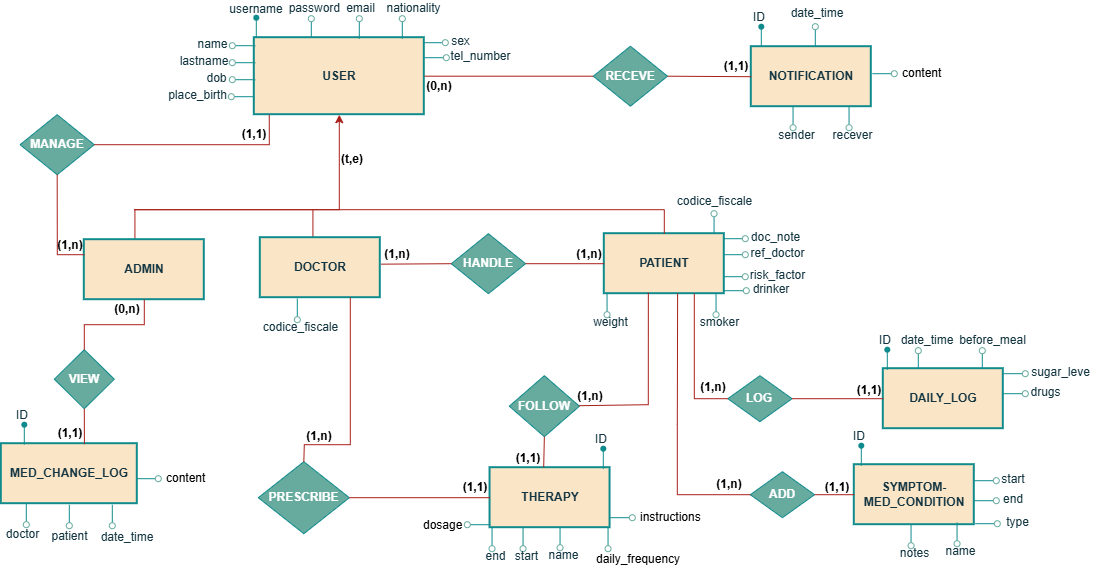
\includegraphics[width=1\linewidth]{VelyaLife_ER-schemas.drawio.png}
        \caption{ER-Schemas}
    \end{figure}

    \subsubsection{Entity Subtyping and Roles}
    Instead of duplicating authentication credentials, the Doctors table and the Patients table act as extensions of the User table, linked via a unique Foreign Key, to handle the distinction between doctors and patients. A streamlined and normalised database architecture is ensured by the attribute
    type on the main user record, which dictates whether the application should fetch the associated doctor's metadata or the patient's one.

    \subsubsection{User registration process}
    When a user is registered to the system they receive an email with username and password. In the utility folder there is the code for the email service. For this service specific java library (jakarta mail/SMTP) was used.

    In same forder you can find some check functions used to verify the correctness of the information inserted such as codice fiscale, email. The algorithm to check codice fiscale was projected based on the rules defined by the italian government, it was tested and works (check the resource section for the implementation). In the how to use section it is stated how to enter information so that these functions work properly.
    
    \subsection{Frontend}
    The frontend is created using the \textbf{JavaFx} framework, which is composed of a structured architecture with a theatrical theme consisting of scenes and stages. Along with CSS styling, Scene Builder was utilized to streamline the building process. 
    
    Following the completion and testing of each backend component, the user interface was constructed. Every piece of visual content (i.e. an e. Icons and pictures) were created with Canva. AI was used to select the name from a list of options.

    \subsection{Difference between versions}
    Lots of changes were made in this new version (backend and frontend). Things that were removed and/or replaced from the old version in this one:
    \begin{itemize}
        \item Horizontal menu bar with profile and login buttons for all users was removed.
        \item Default language is english and not italian.
        \item All the images are replaced using the ones I made in Canva.
        \item Password column was removed from patient and doctor list. In exchange name and last name columns were added.
        \item User sign up form was changed. The needed information to insert change based on the user's role. Codice fiscale and email checks have been implemented.
        \item In patient's profile, they can view and change information.
        \item Message list table has date, sender columns added. It also has a button if the message hasn't been viewed yet.
        \item In the therapy detail section it is written which doctor wrote that medication. It is also provided the period in which they have to follow that therapy.
        \item In the daily log sections I have added a section to insert symptoms and/or medical conditions. Daily log limit was removed.
        \item Alert system has been changed.
    \end{itemize}
    New features present in this version are:
    \begin{itemize}
        \item For the patients a summery section (My chart) was added.
        \item For doctors, their patient detail page has been added.
        \item Both doctors and patient cha download their medical chart.
        \item Every user receives an email in case of profile update and/or elimination.
        \item Patients get a remainder to follow their therapy.
    \end{itemize}
    
    \section{Tests} 
    VelyaLife's testing approach is bottom-up and modular. To guaranty functional correctness, each component—such as database schemas and user interface elements—was tested separately. Following the success of these unit tests, the components were incorporated into more comprehensive modules to confirm their overall behavior. As the system became more complex, this approach allowed interface errors to be caught early and ensured that the core logic of the application continued to work.
    
    All test scripts are located in the \texttt{/tests} directory within the source code.

    \section{How to Use}
    \subsection{Requirements}
    \begin{itemize}
        \item Any OS works
        \item Java IDE: for this project \textbf{intellij} was used. The original project was made using eclipse.
        \item Database management system: SQLite was used for both this version and the original version.
        \item Email provider for the admin (use an external file since they are sensible information)
    \end{itemize}
    \subsection{Installation Process}
    Set up your desired database and email service. After configuring the IDE you selected, copy the project there and open the file named \textbf{Launcher} and click run. If everything works you'll see the home page.

    In the resource section there are all the link to every tool used for this project.
    
    \subsection{App}
    The home page has a login button which will take you to the relative page. At the top of the page there is a menu bar. Based on where you are it allow you to go to the home page or the login one.
    \begin{figure}[H]
        \centering
        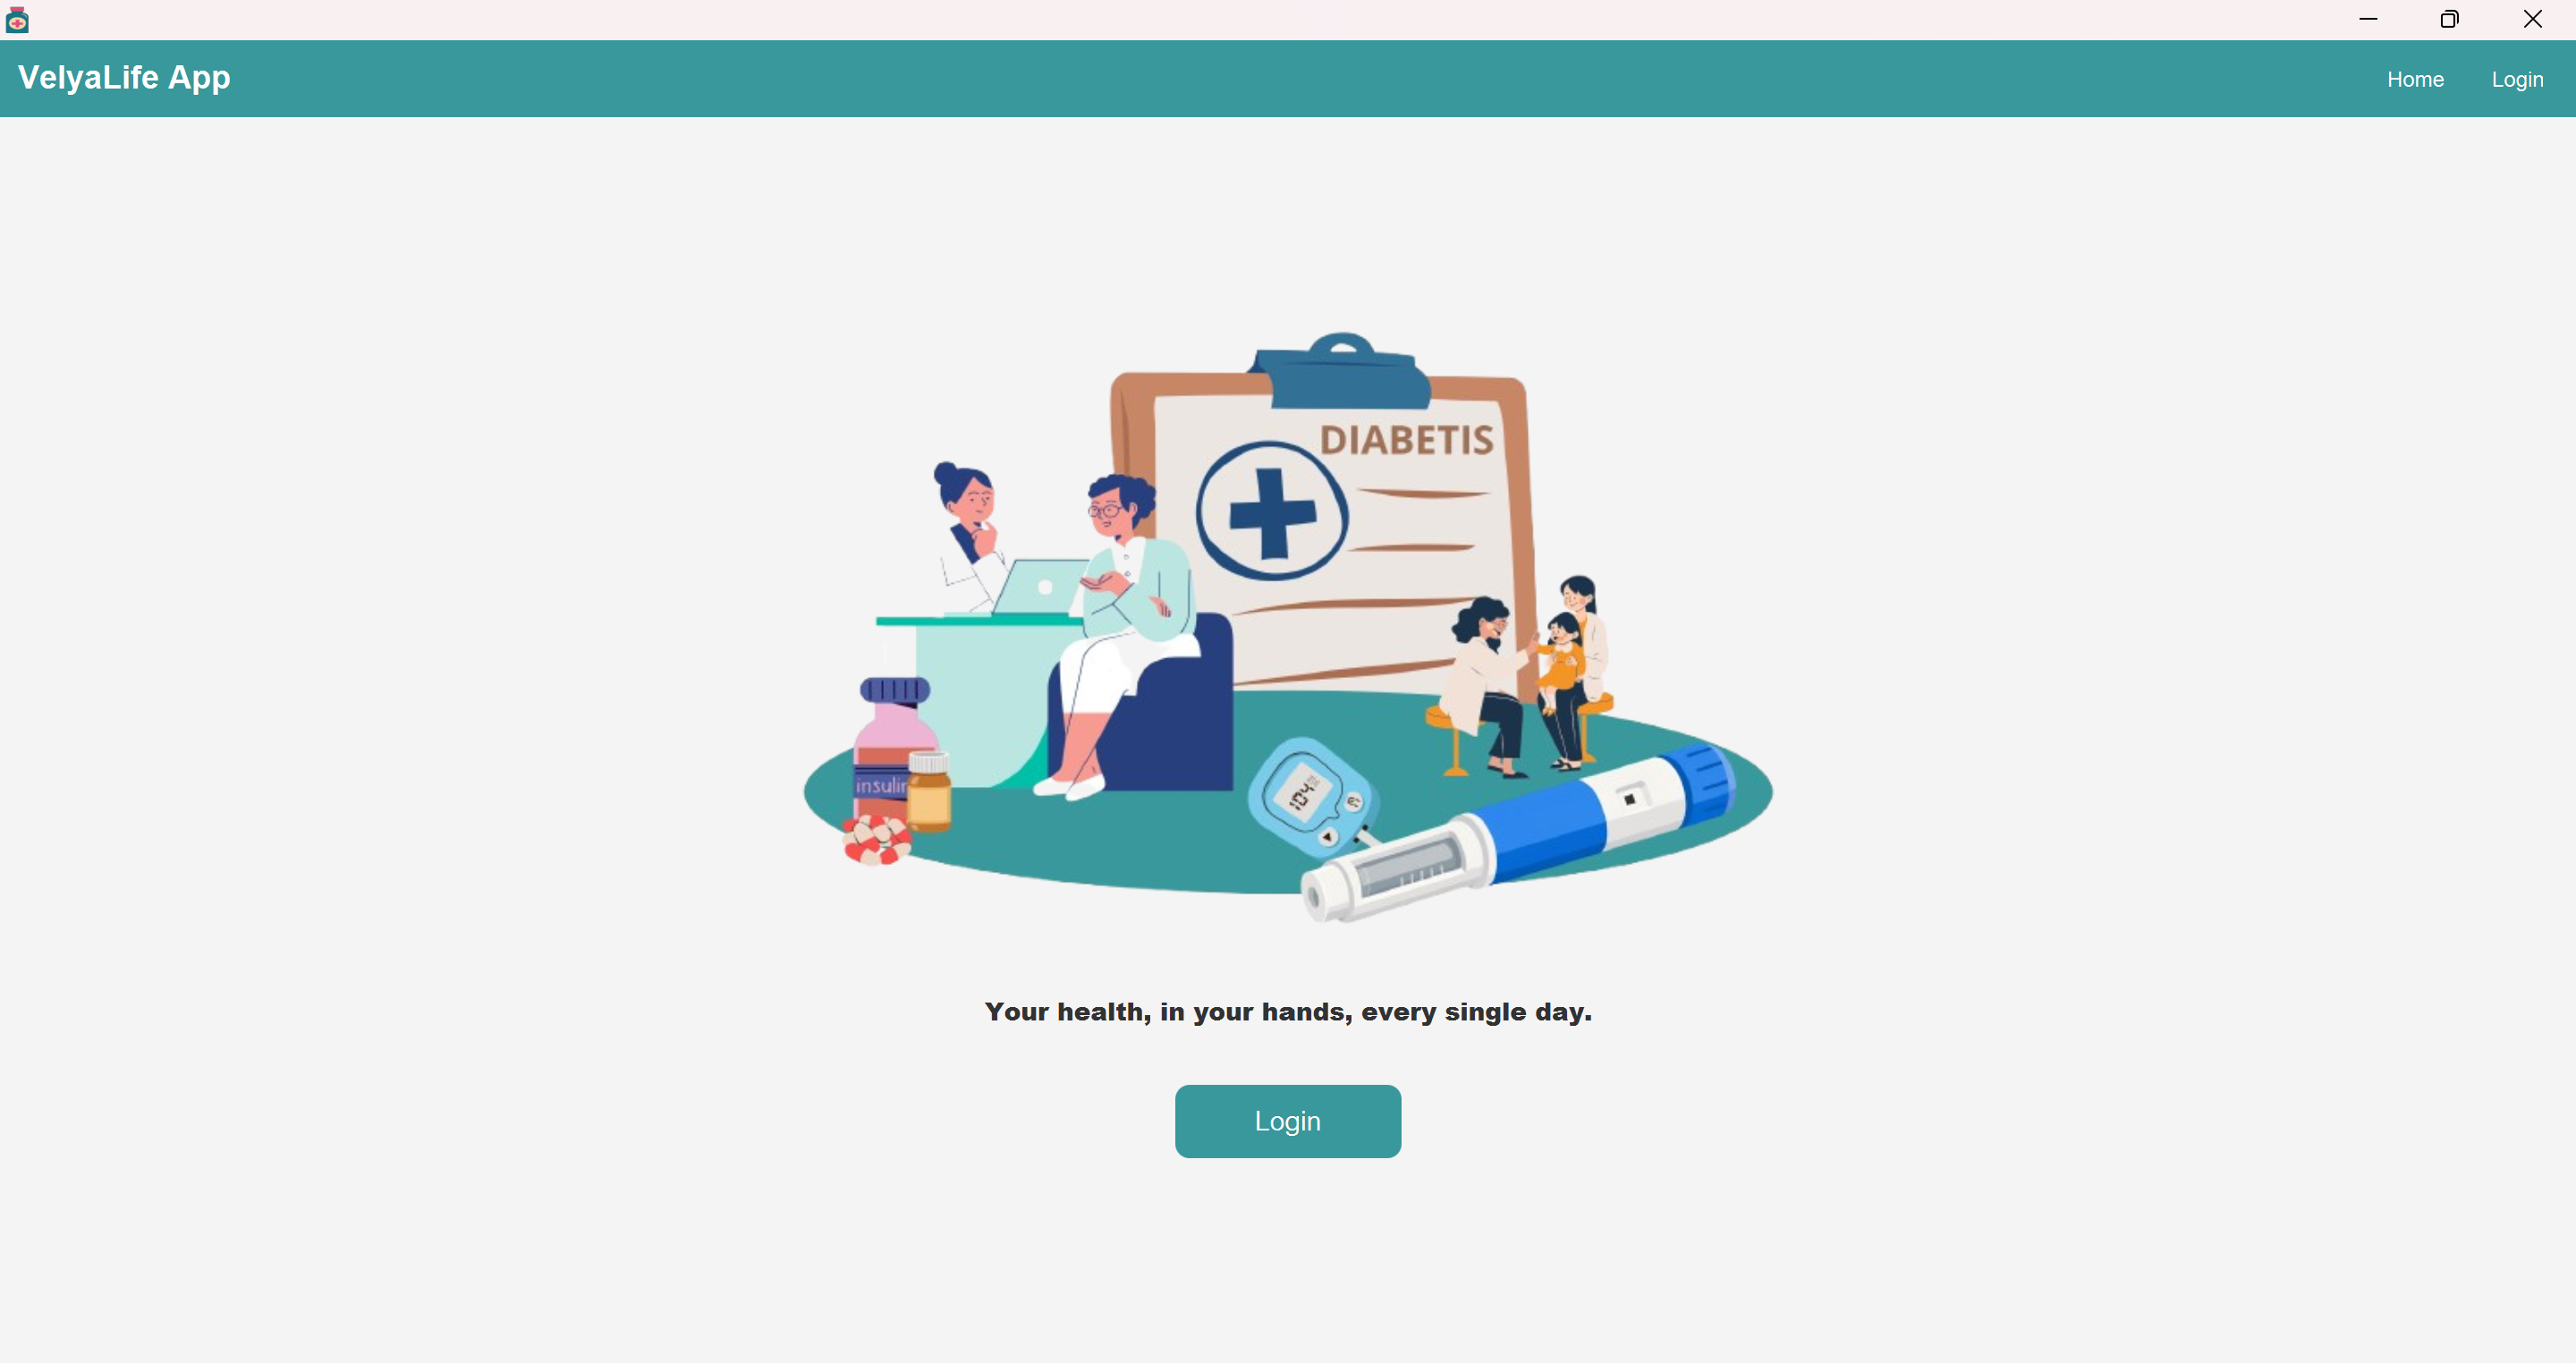
\includegraphics[width=1\linewidth]{home_page.png}
        \caption{Home screen}
    \end{figure}

    Click on the login button. It will take you to the login page (the admin has already registered the user, so there is no registration process before the start). Insert username, password and select the user type (admin, patient, doctor) then click login. If you click on show password you will see your password in clear.
    \begin{figure}[H]
        \centering
        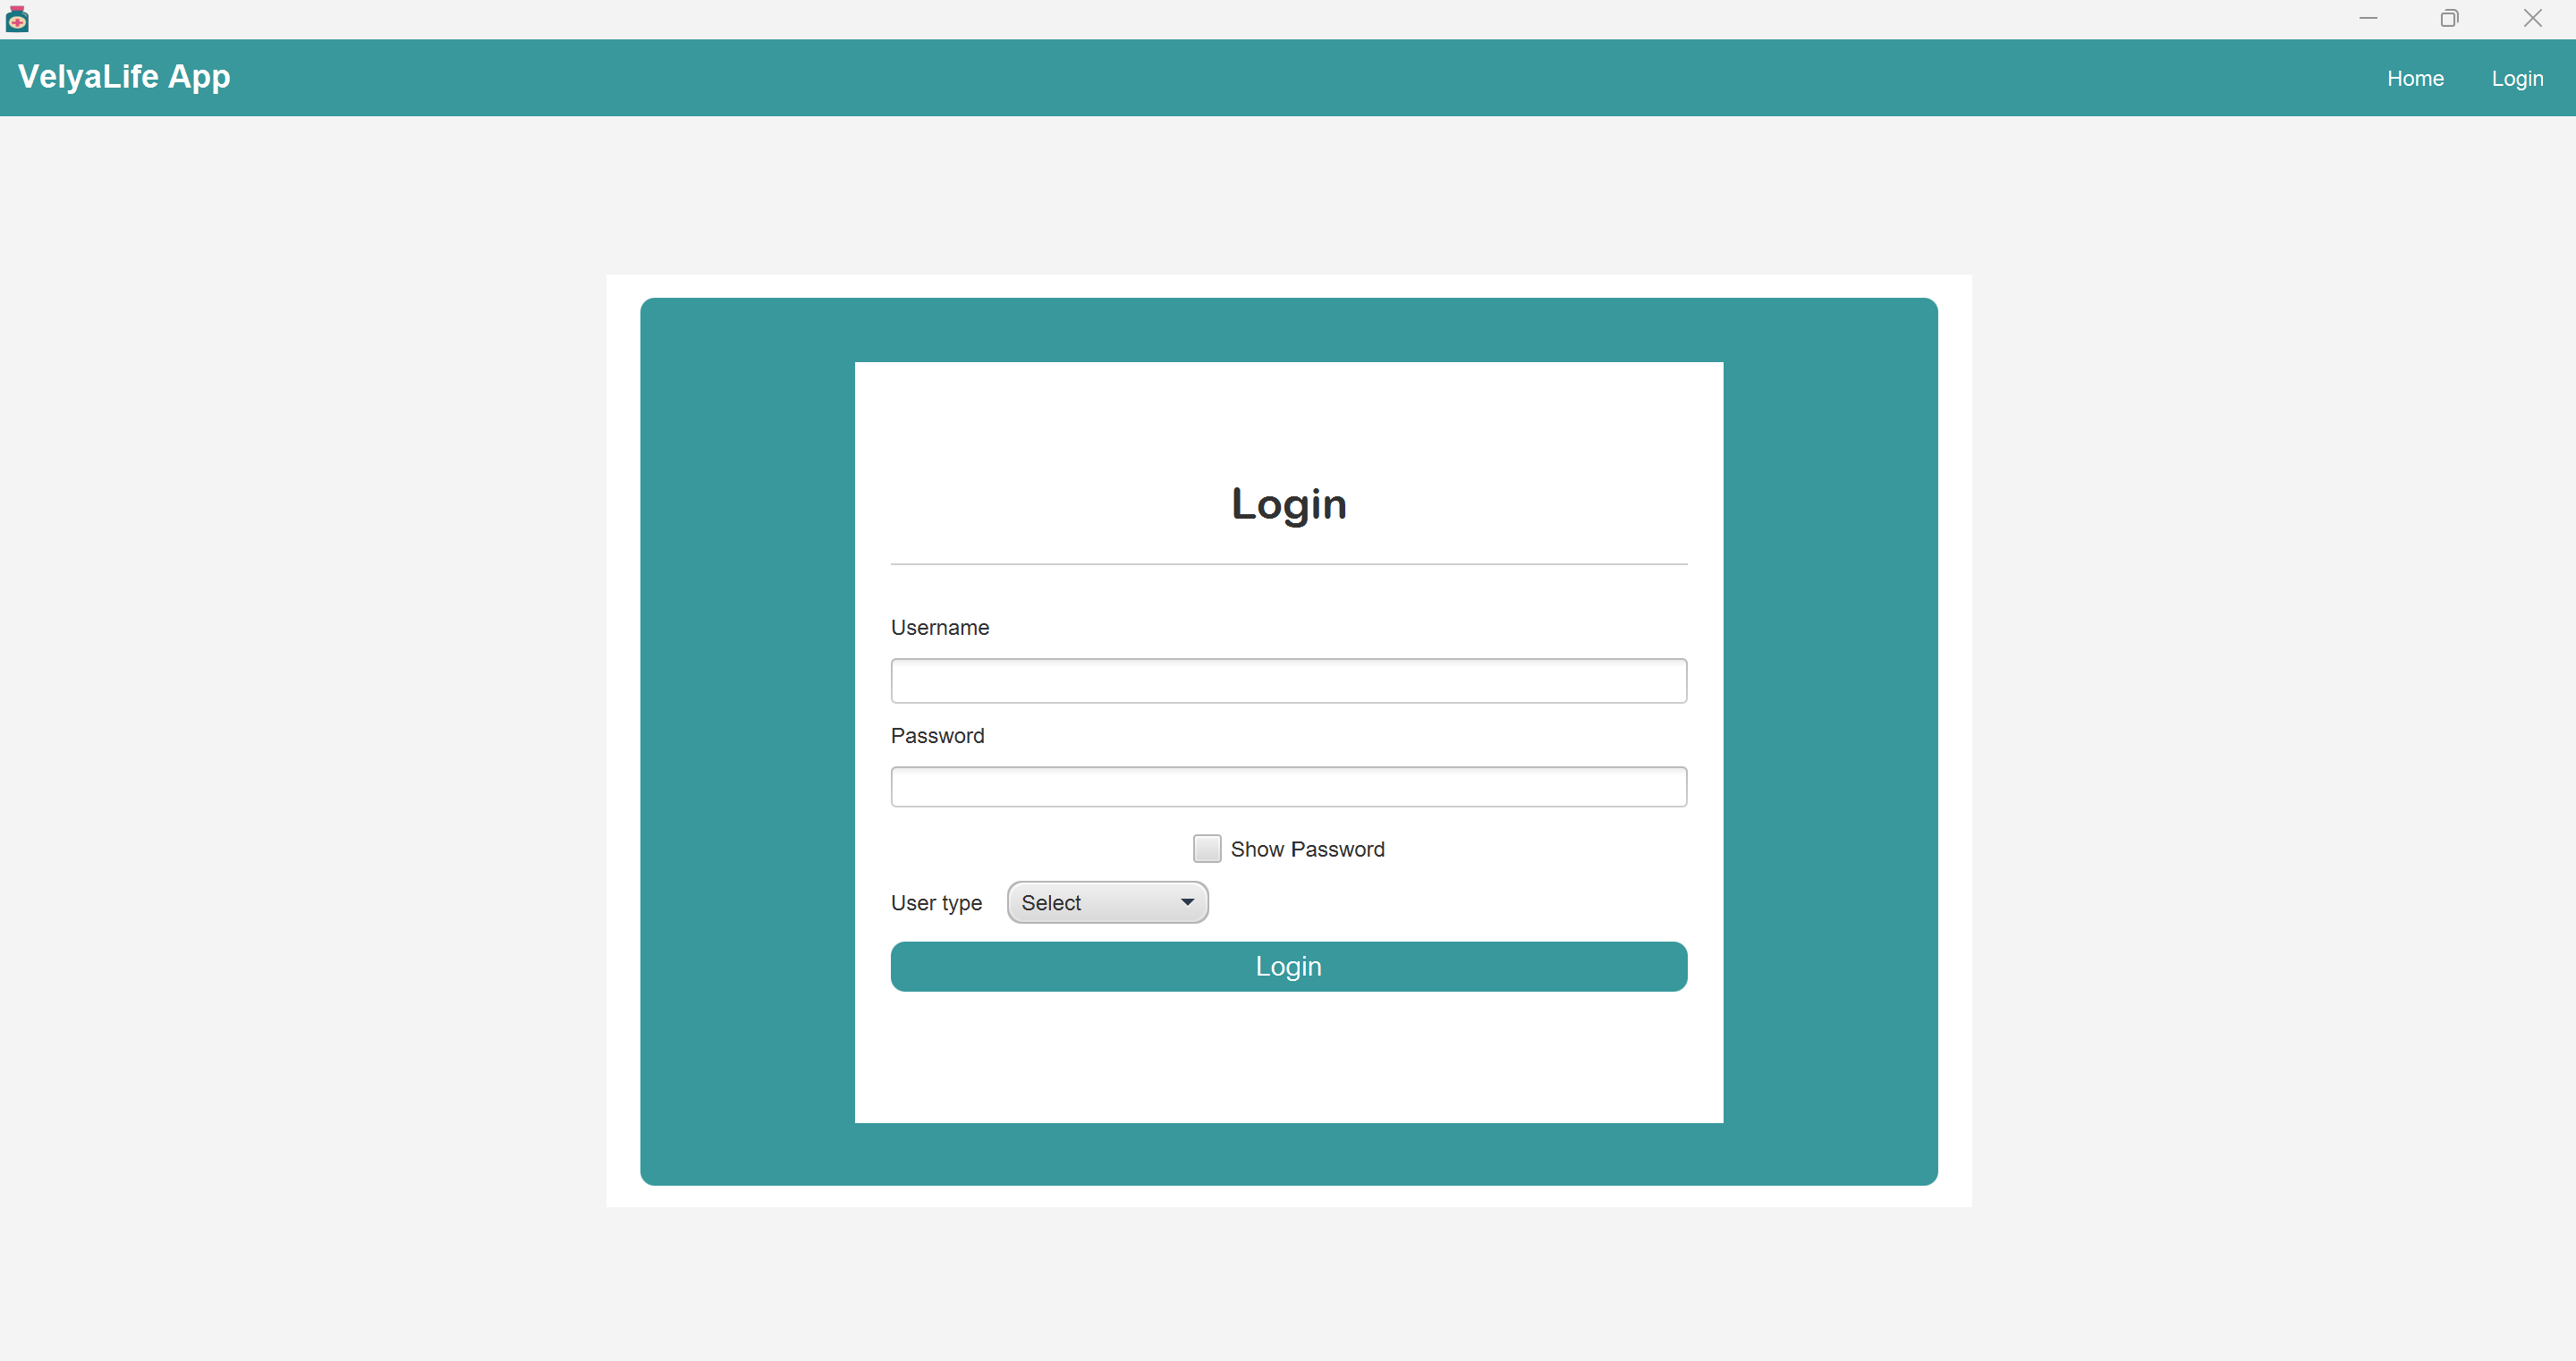
\includegraphics[width=1\linewidth]{login_page.png}
        \caption{Login page}
    \end{figure}

    Based on the user type you will be redirected to you personal dashboard. All users have a sidebar menu with extra buttons to their profile, dashboard and logout. Admin's Dashboard has user management sections divided in patient list and doctor list, and doctor's activity logs.
    \begin{figure}[H]
        \centering
        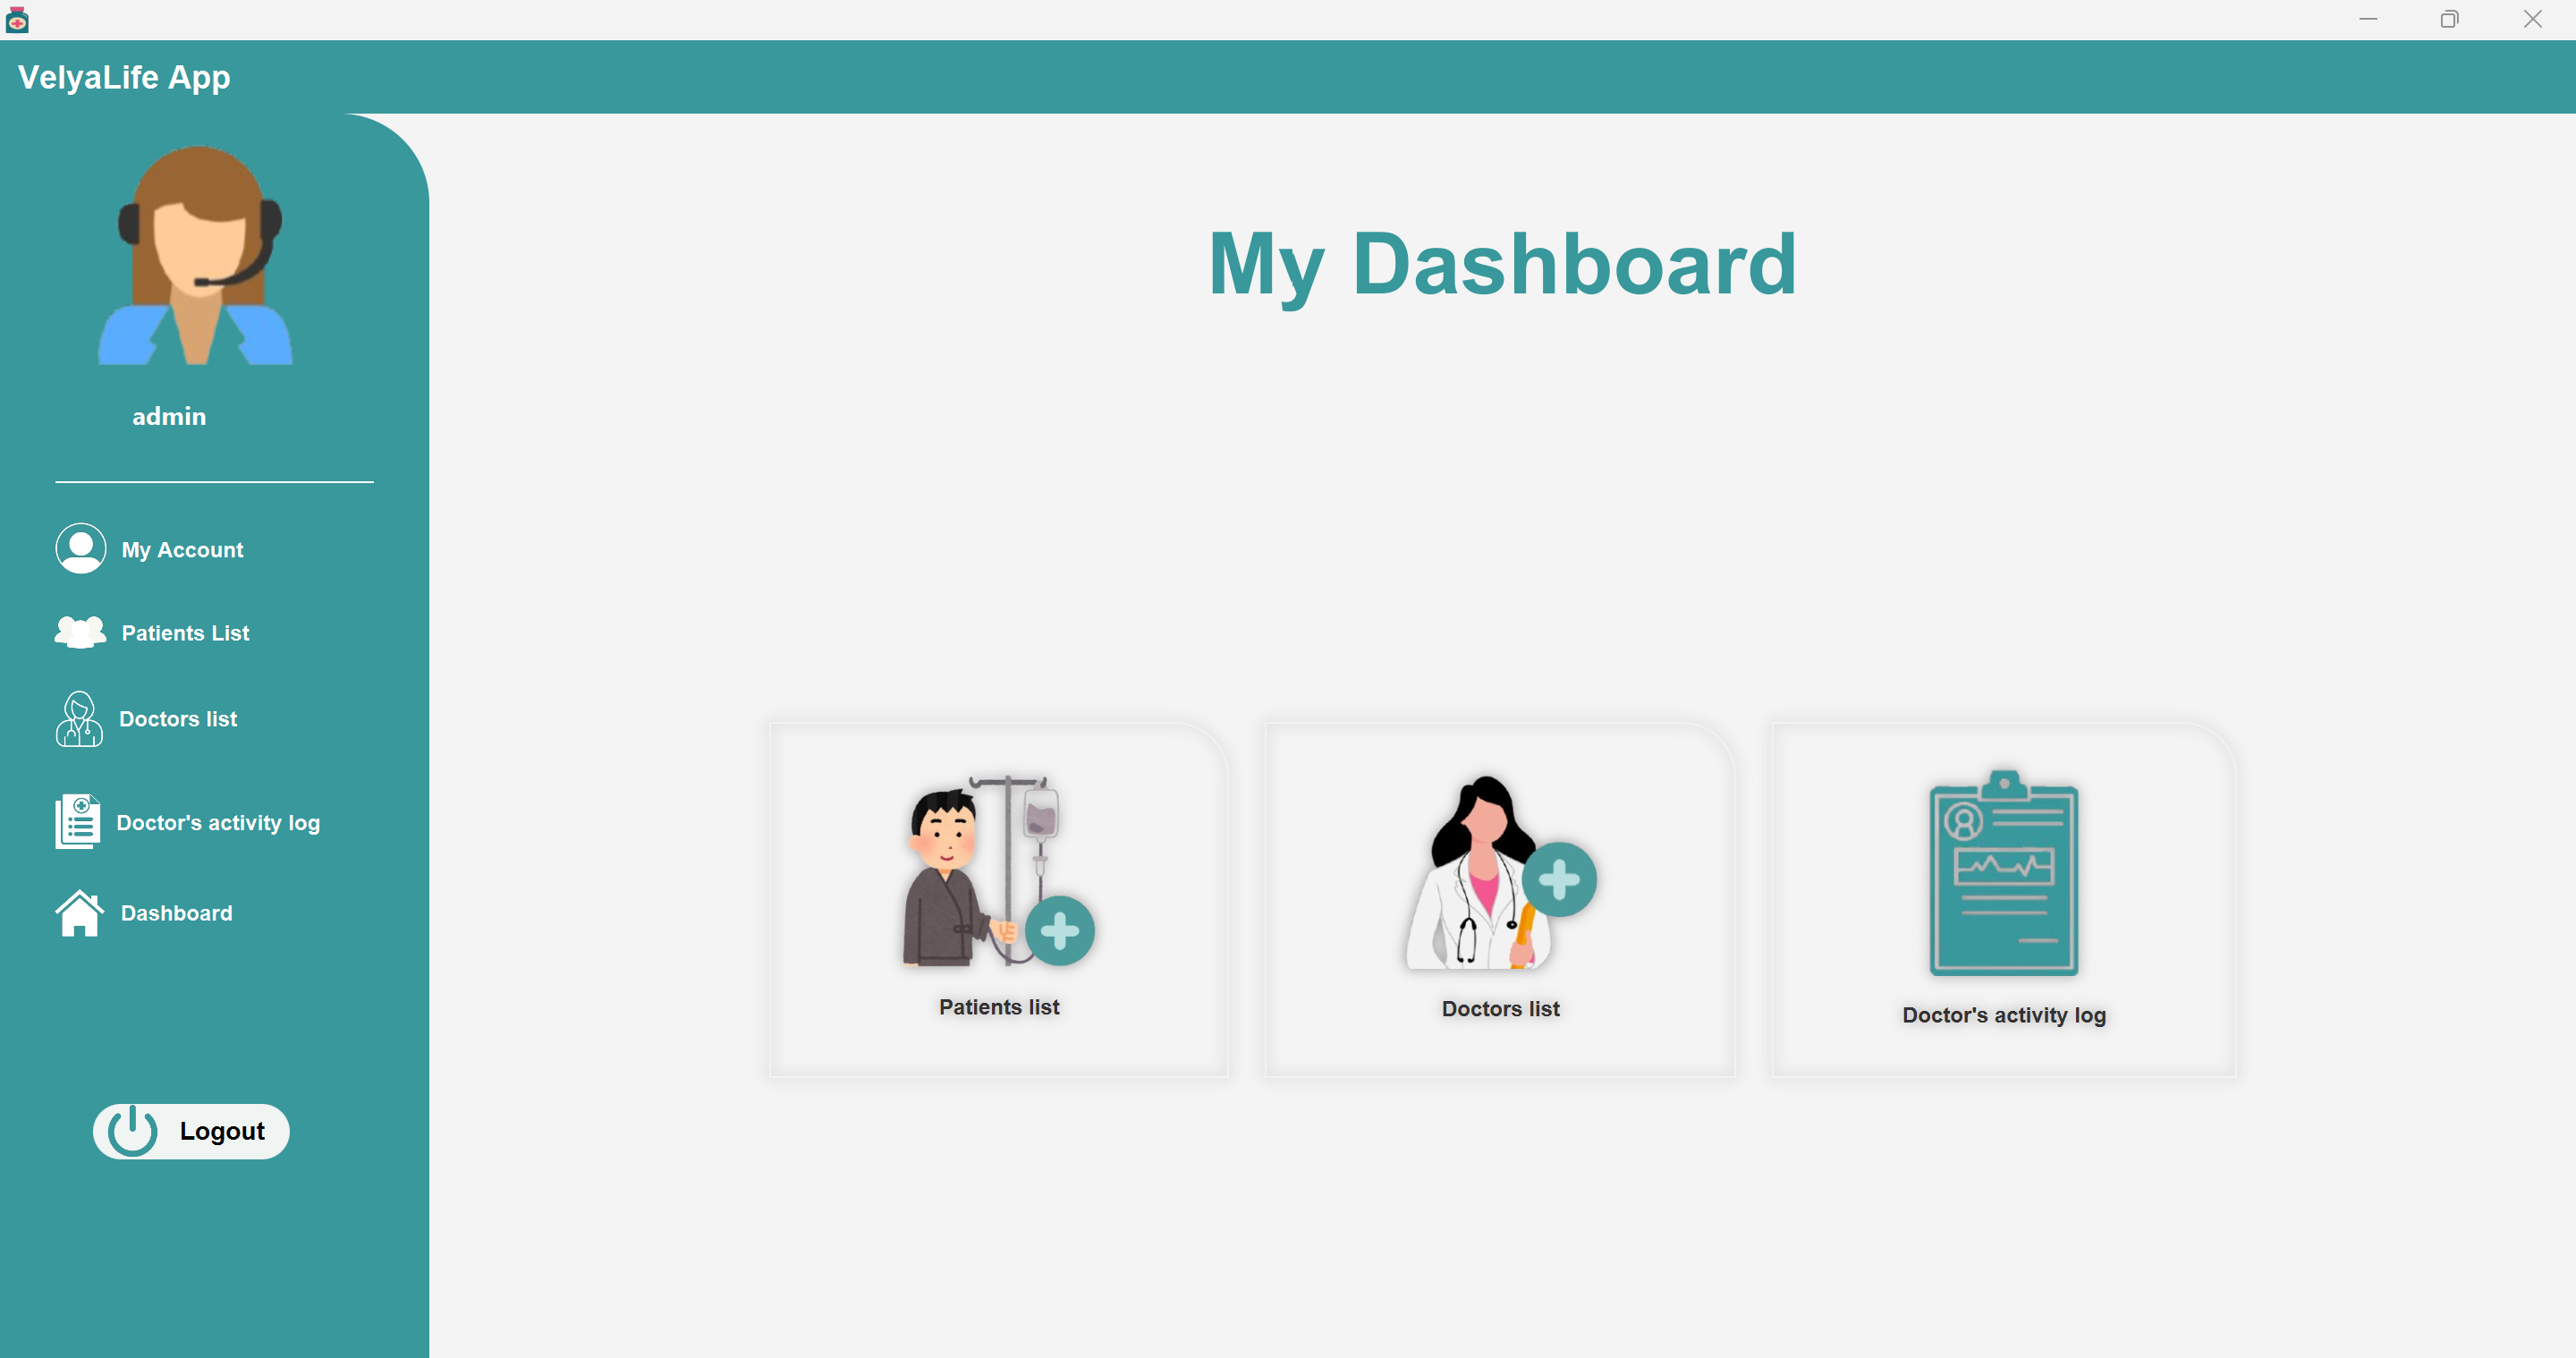
\includegraphics[width=1\linewidth]{admin_dashboard_page.png}
        \caption{Admin's dashboard}
    \end{figure}

    Patient and doctor's dashboards are structured the same way:
    \begin{figure}[H]
        \centering
        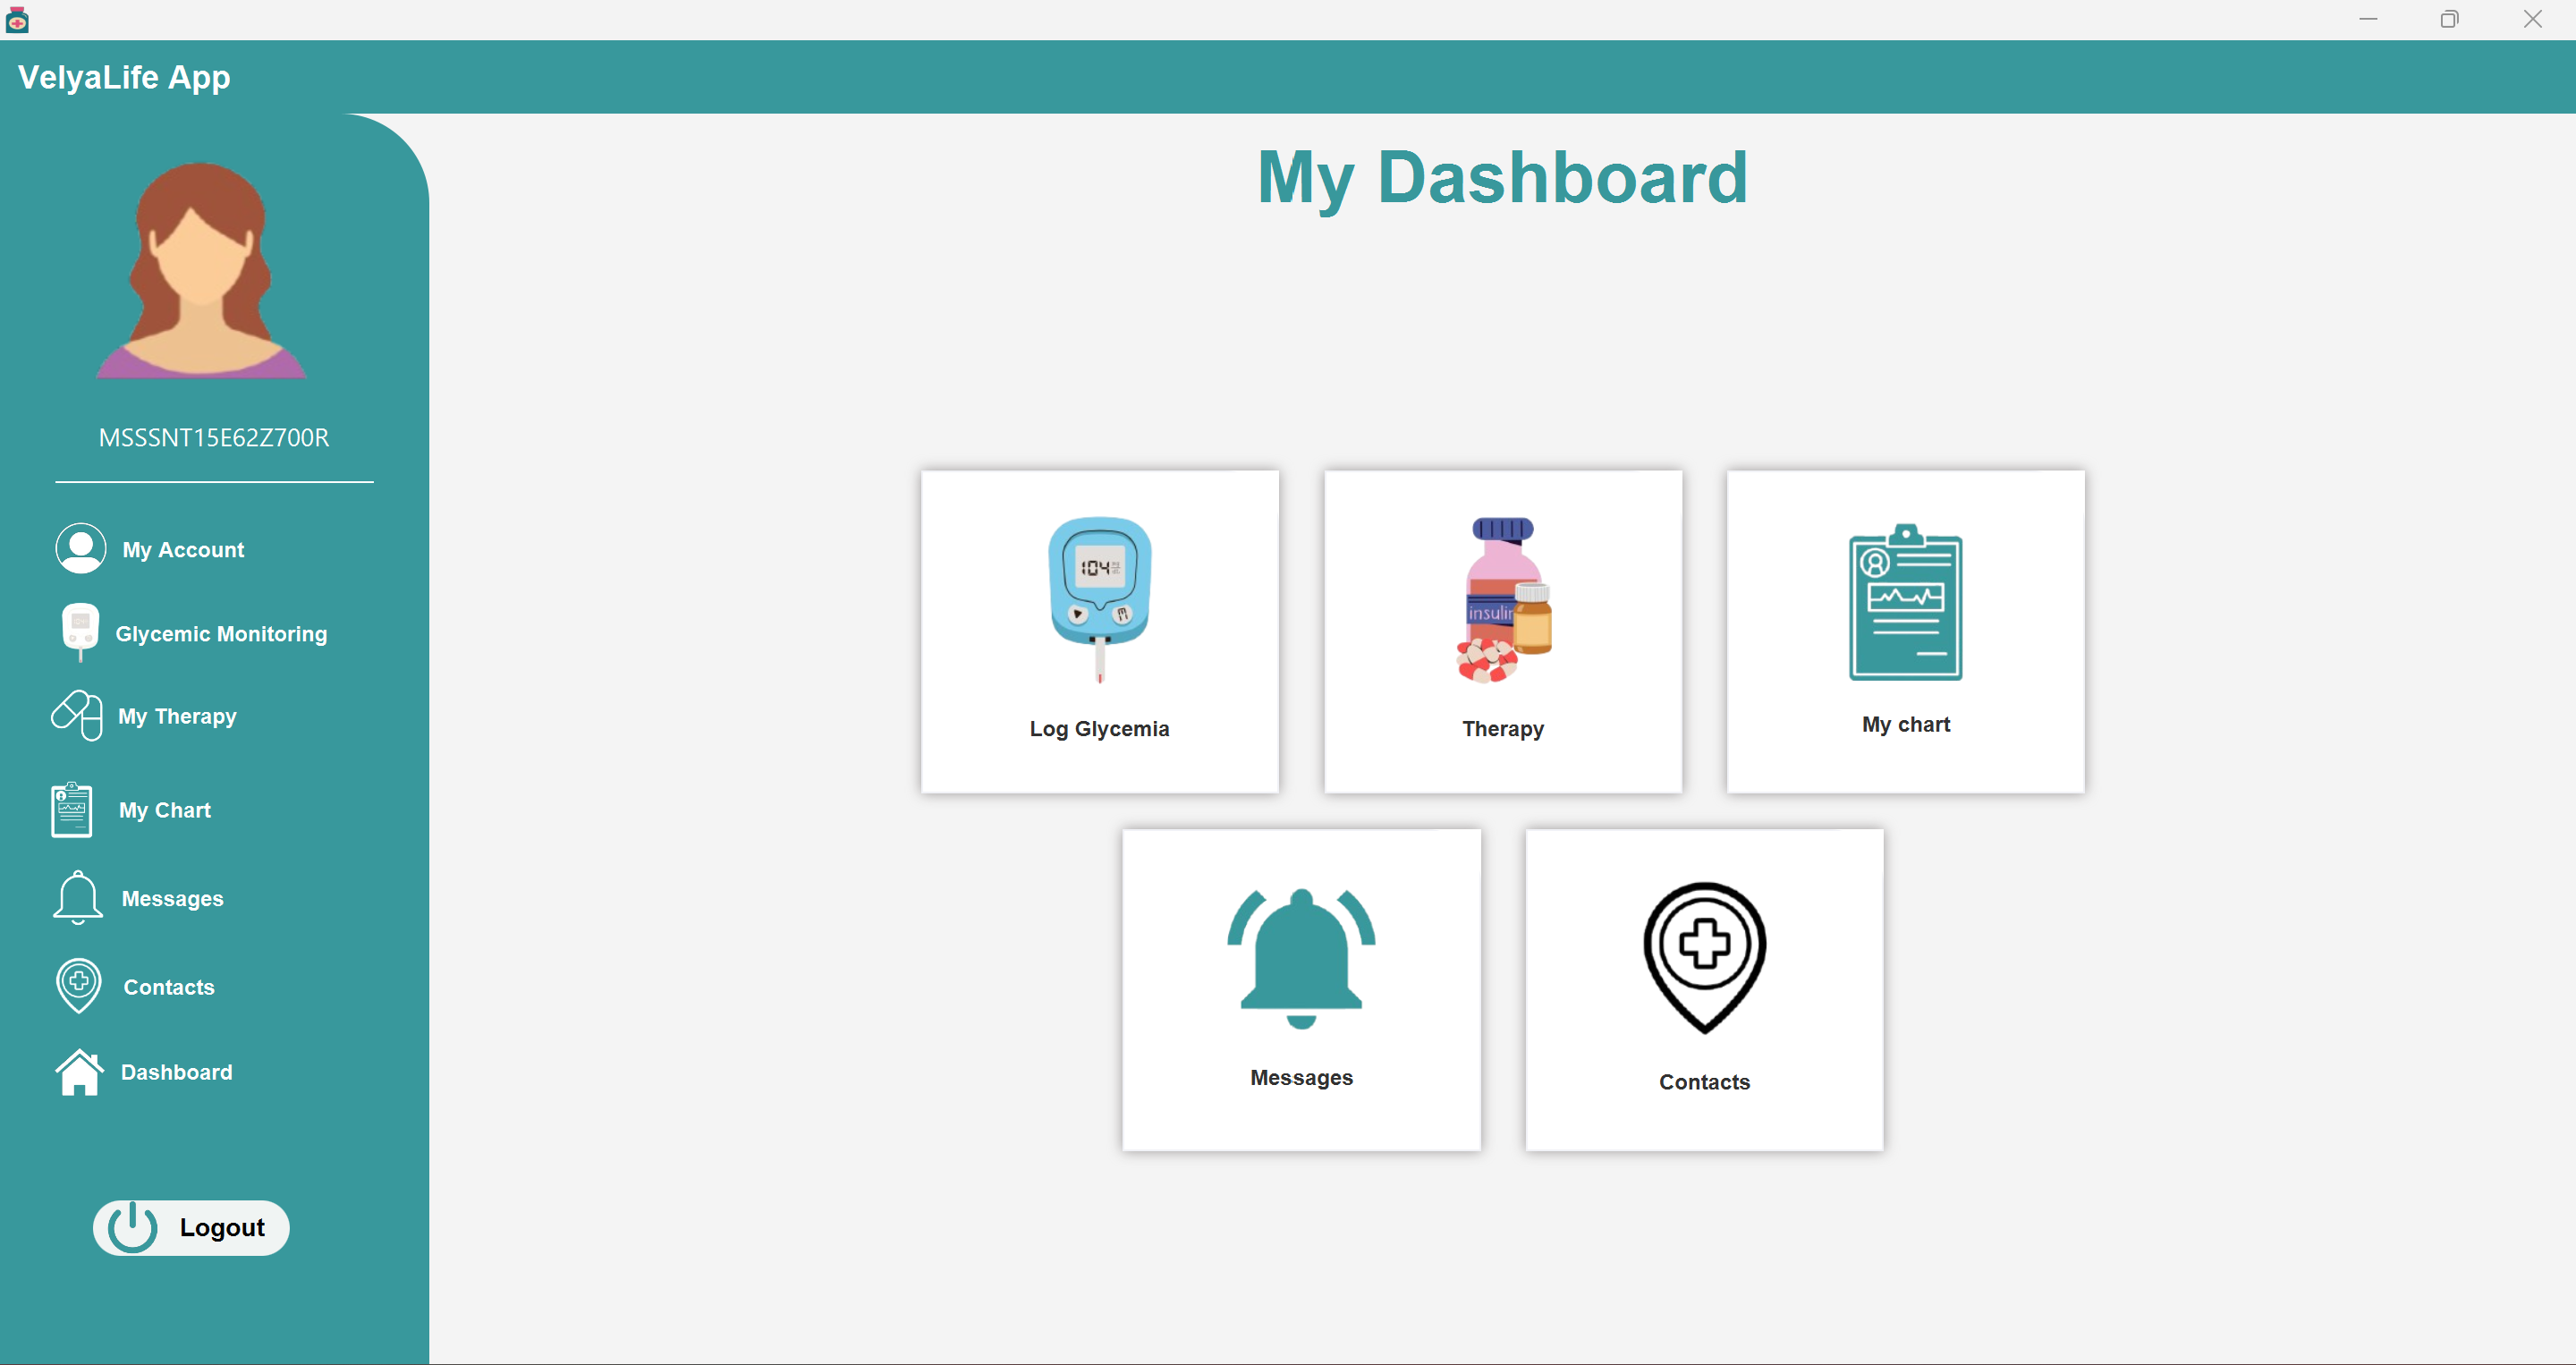
\includegraphics[width=1\linewidth]{patient_dashboard_page.png}
        \caption{Patient's dashboard}
    \end{figure}
    \begin{figure}[H]
        \centering
        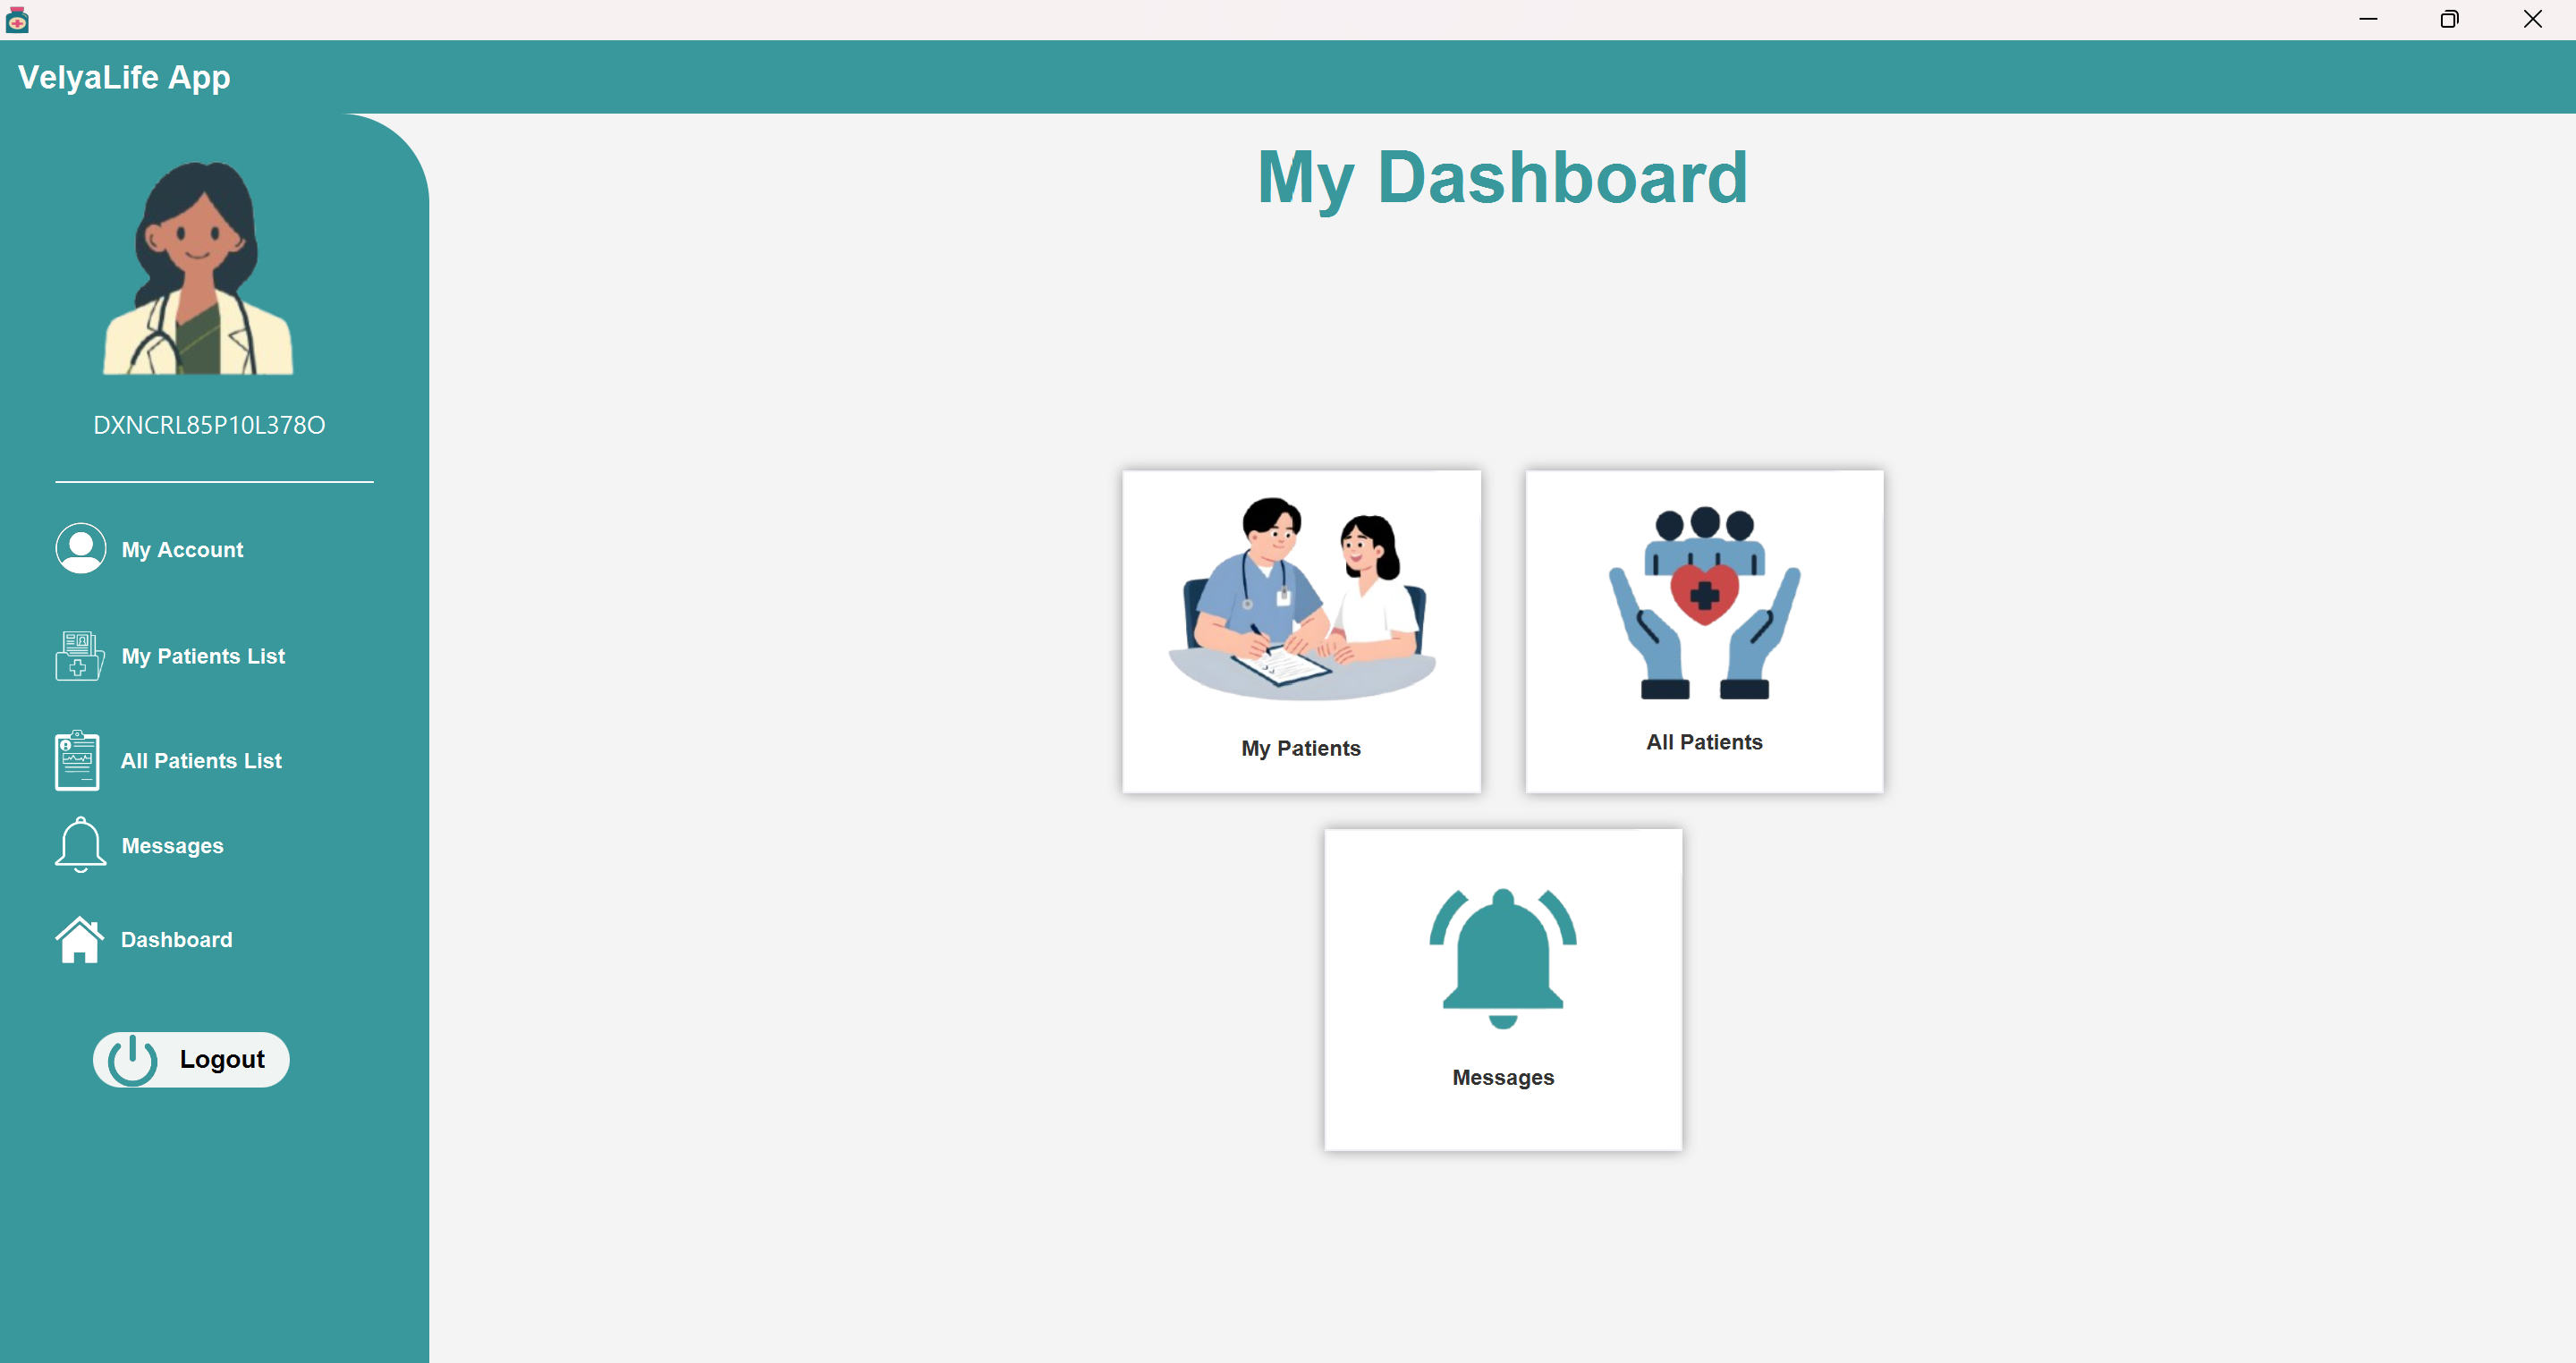
\includegraphics[width=1\linewidth]{doctor_dashboard_page.png}
        \caption{Doctor's dashboard}
    \end{figure}

    Within the source code, there is a file called 'Simulation.txt'. It contains all the information about the users to see how it works.

    \subsubsection{Admin's dashboard}
    The admin can register and delete users. He views patients and doctors separately.
    \begin{figure}[H]
    \begin{subfigure}{0.5\textwidth}
    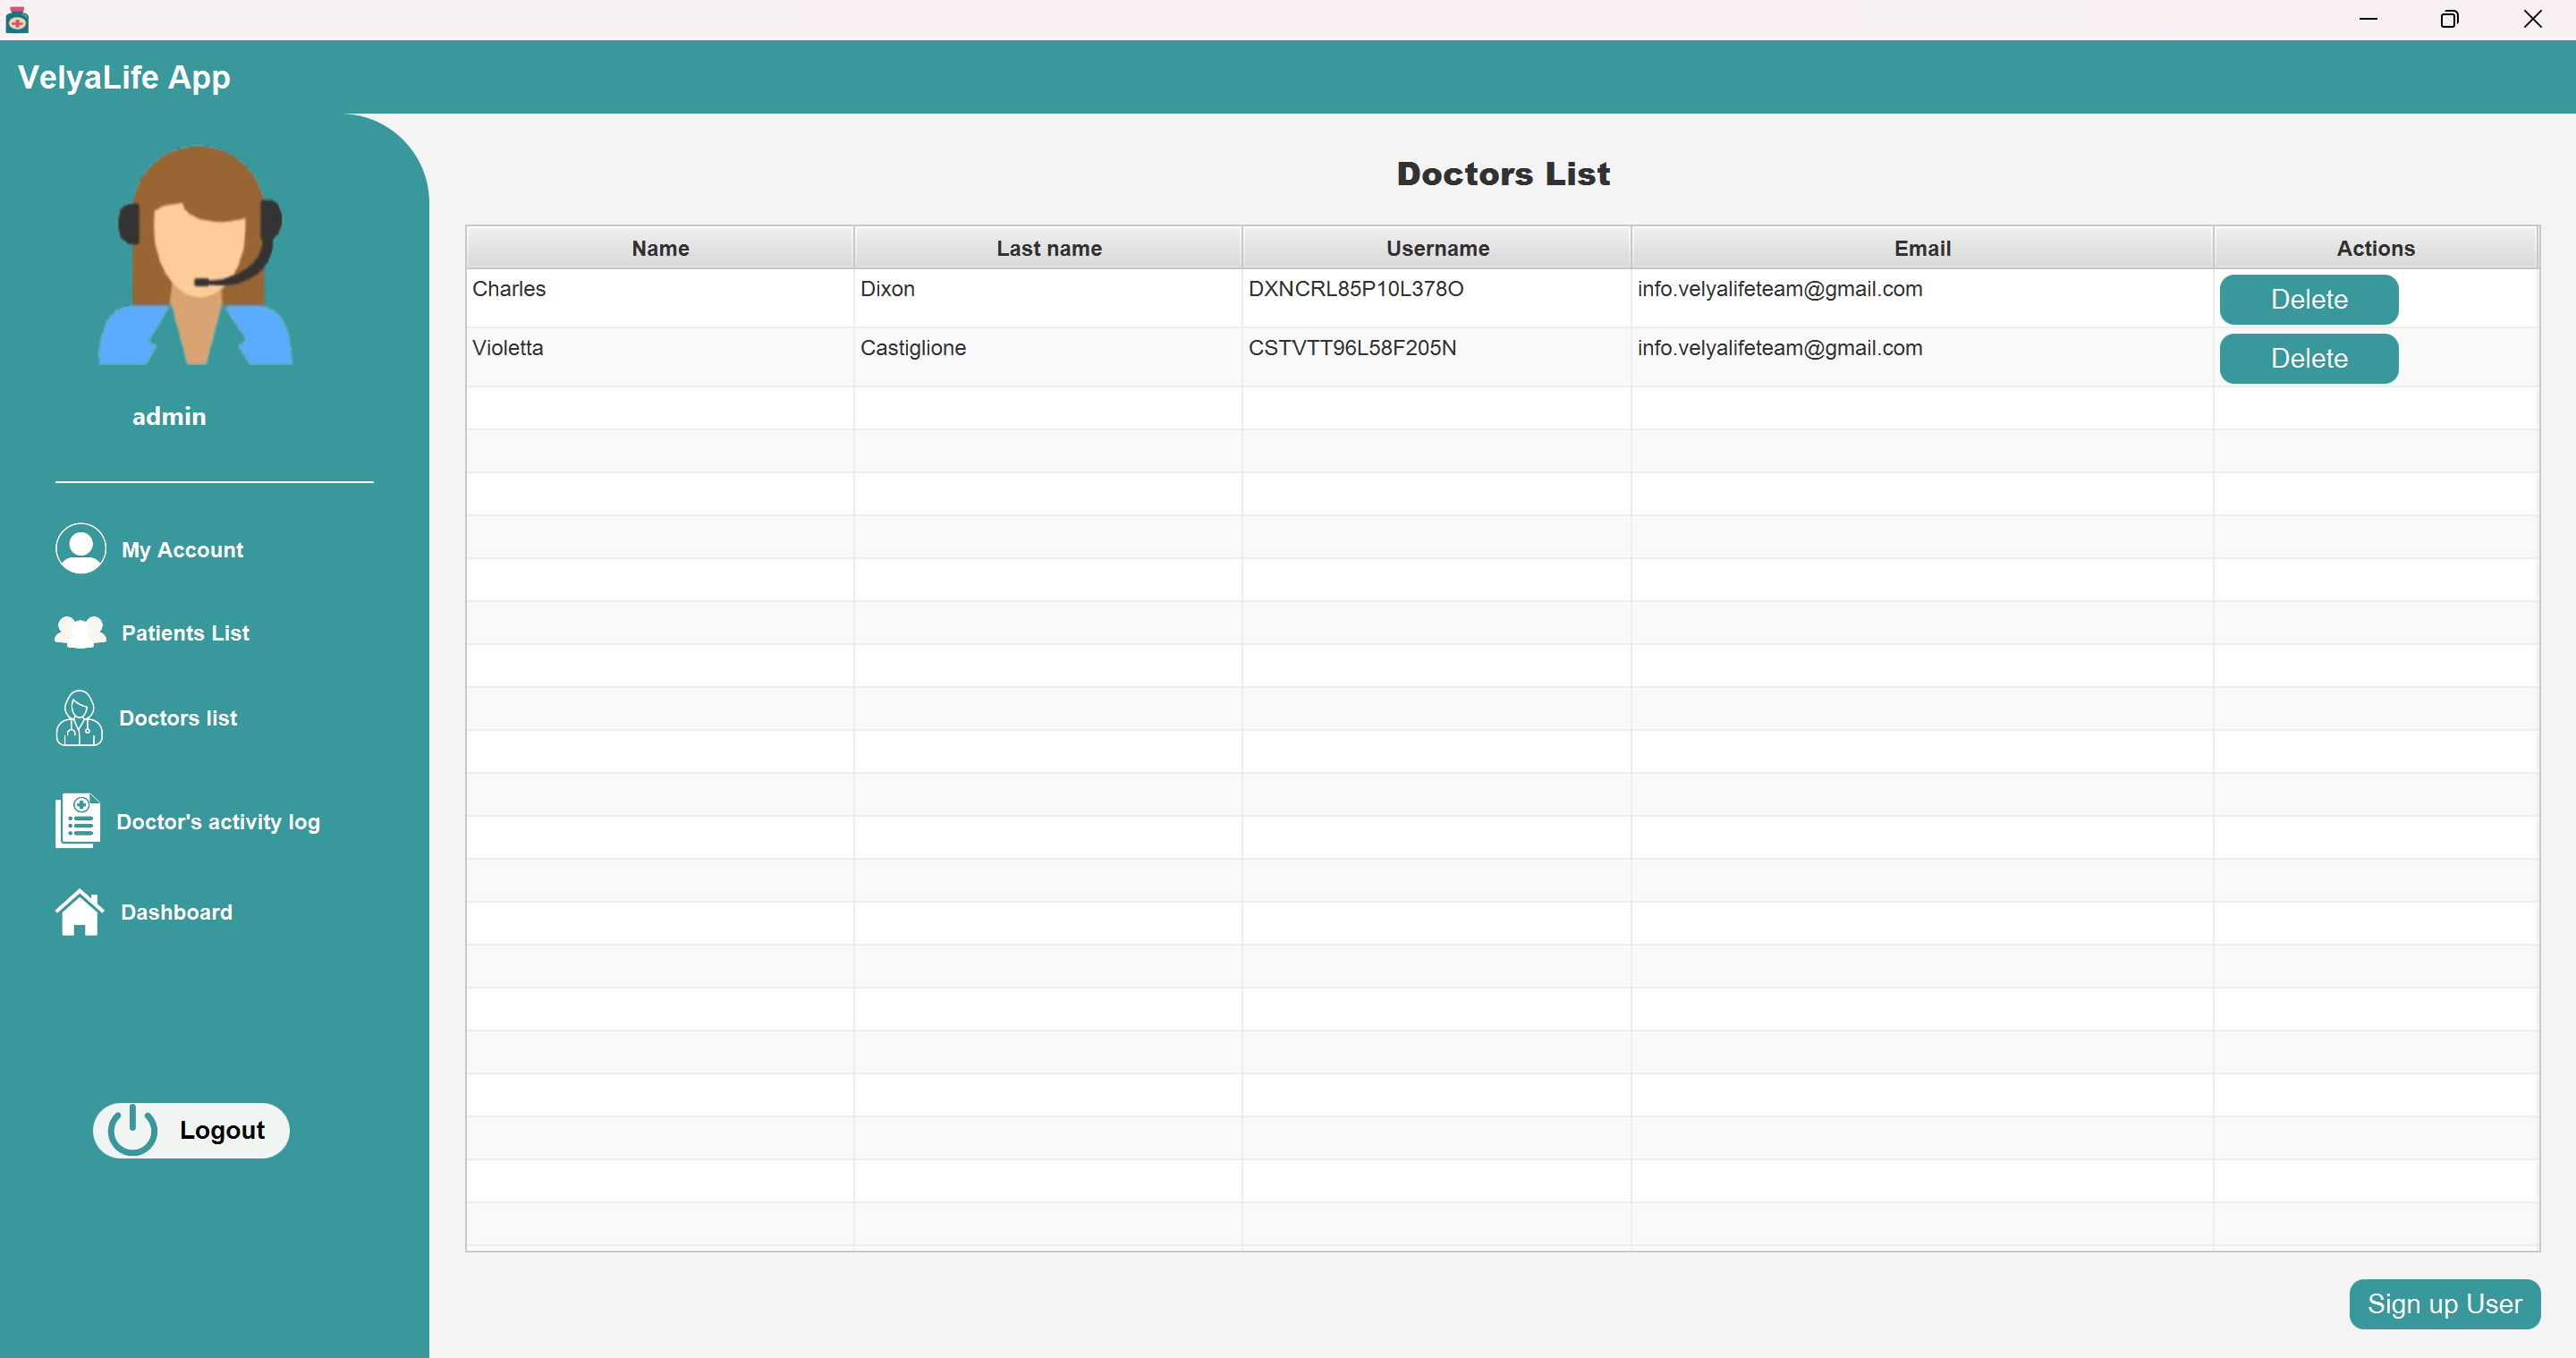
\includegraphics[width=0.9\linewidth, height=6cm]{doctor_list_page.png} 
    \caption{Doctor list table}
    \label{fig:subim1}
    \end{subfigure}
    \begin{subfigure}{0.5\textwidth}
    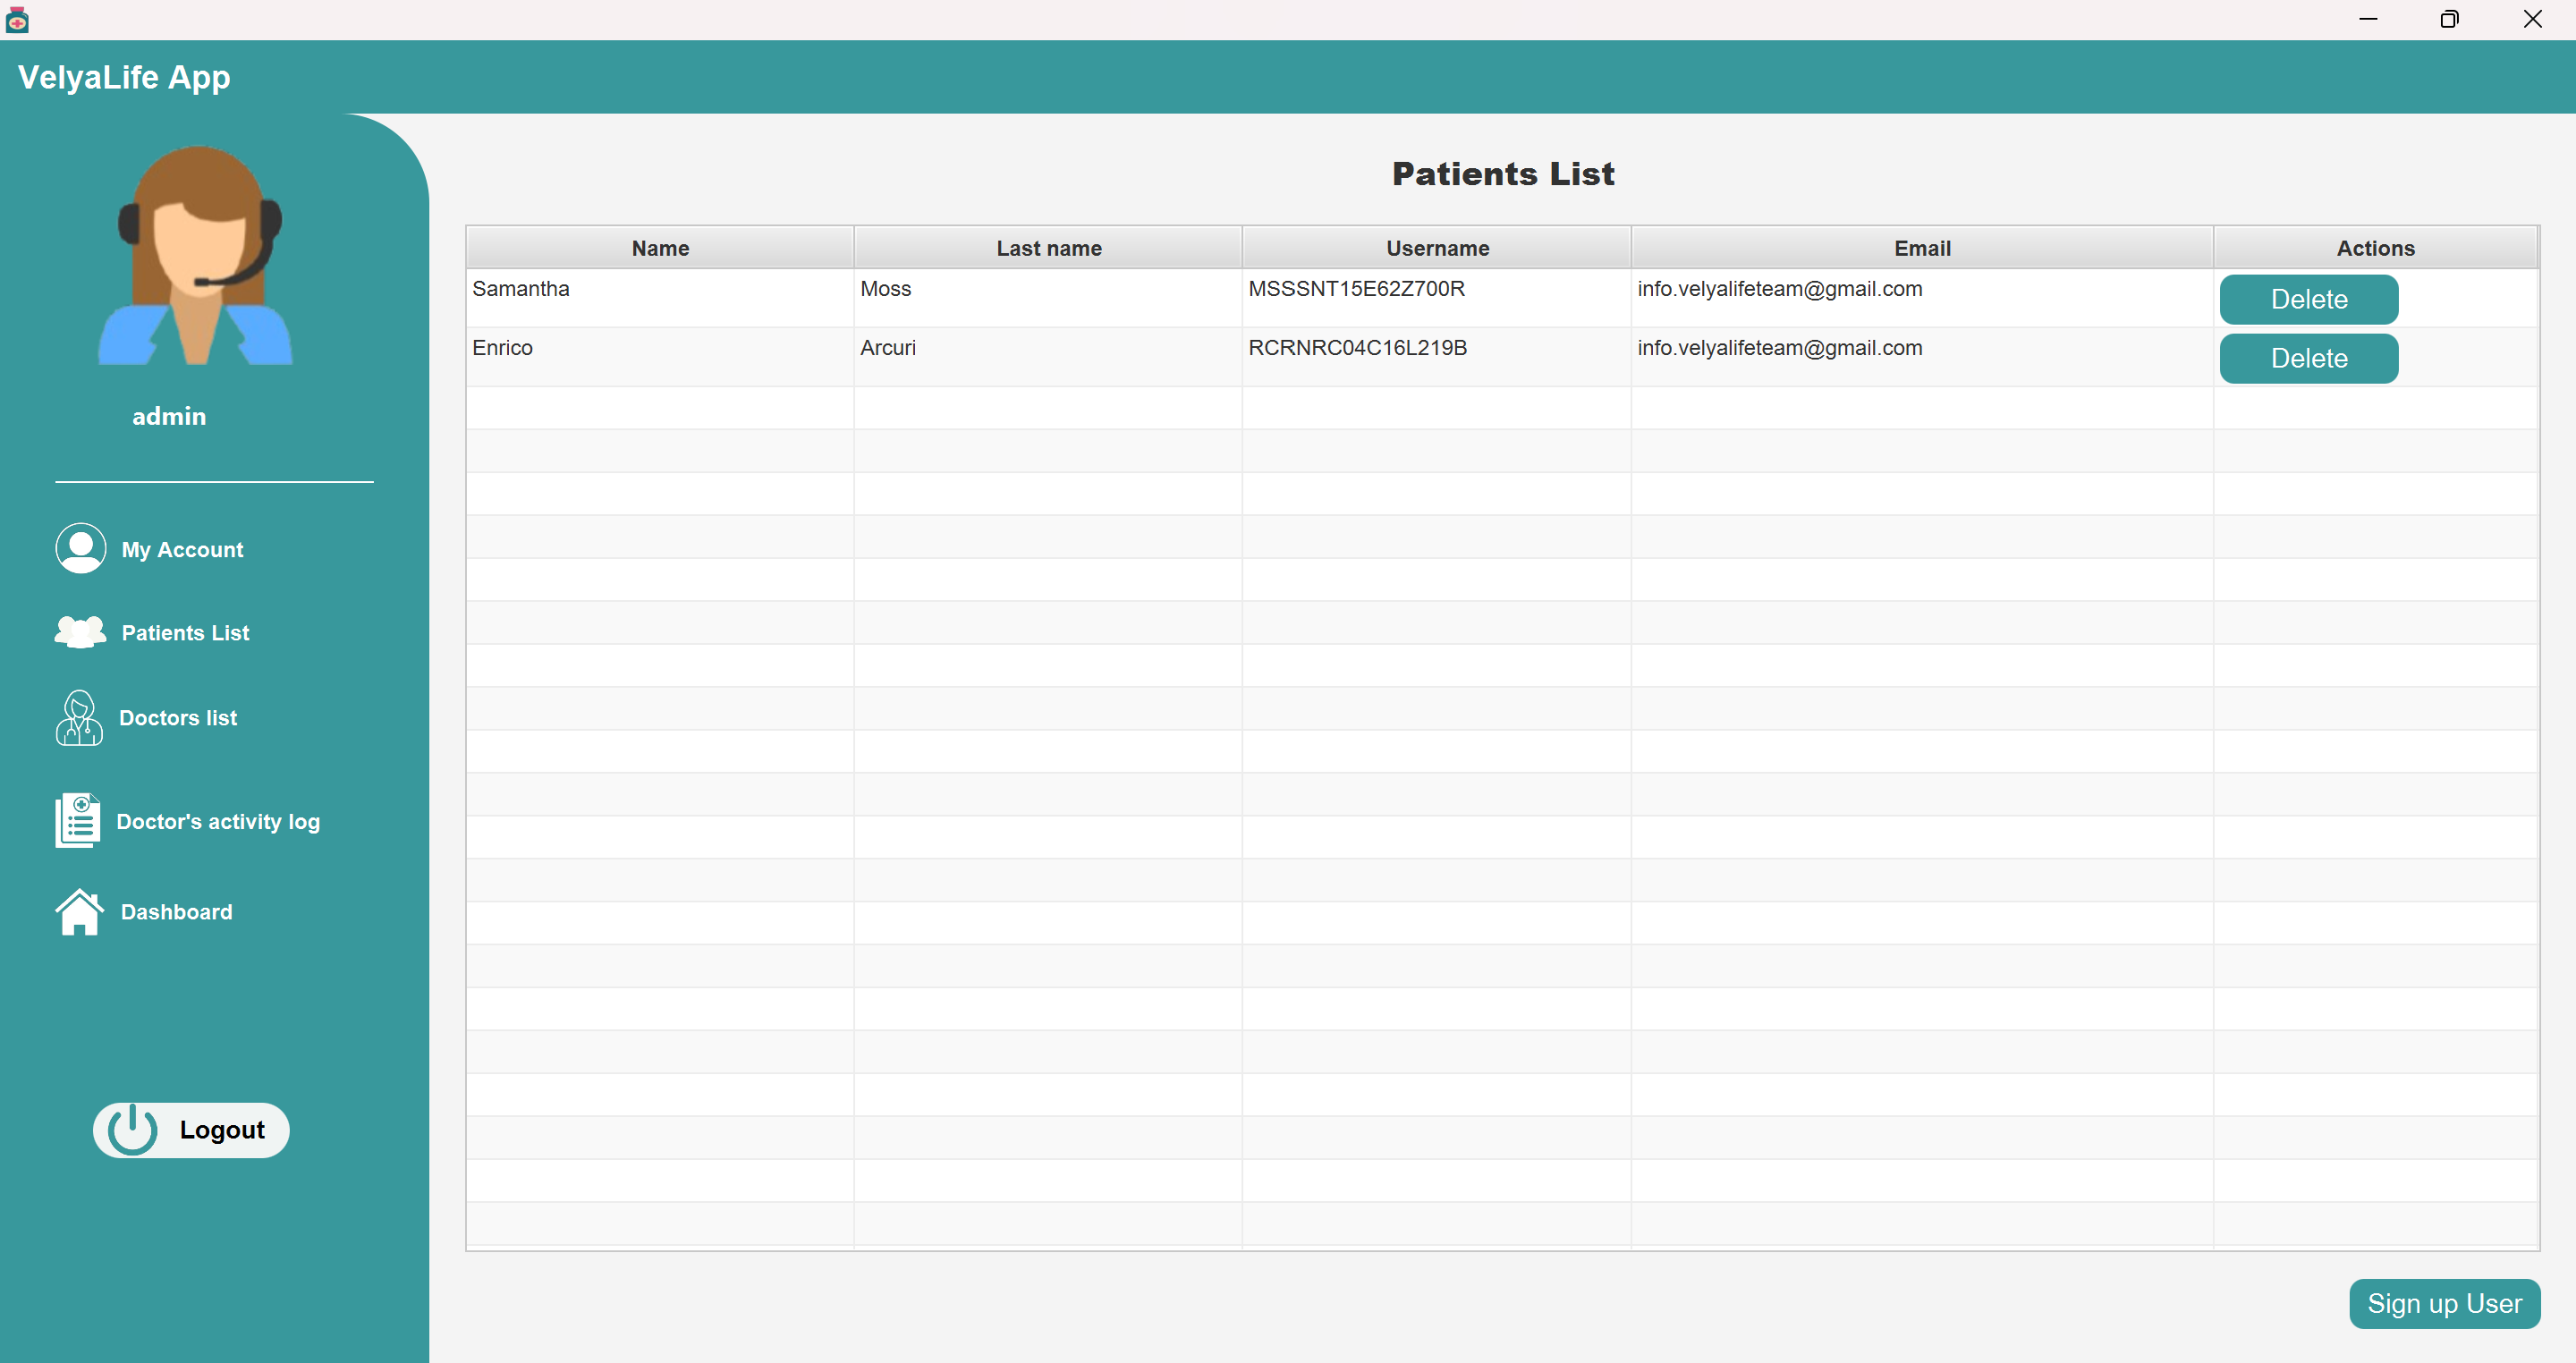
\includegraphics[width=0.9\linewidth, height=6cm]{patient_list_page.png}
    \caption{Patient list table}
    \label{fig:subim2}
    \end{subfigure}
    \caption{User management sections}
    \label{fig:image2}
    \end{figure}

    If you click on sign up user it will take you to the registration section.
    \begin{figure}[H]
    \begin{subfigure}{0.5\textwidth}
    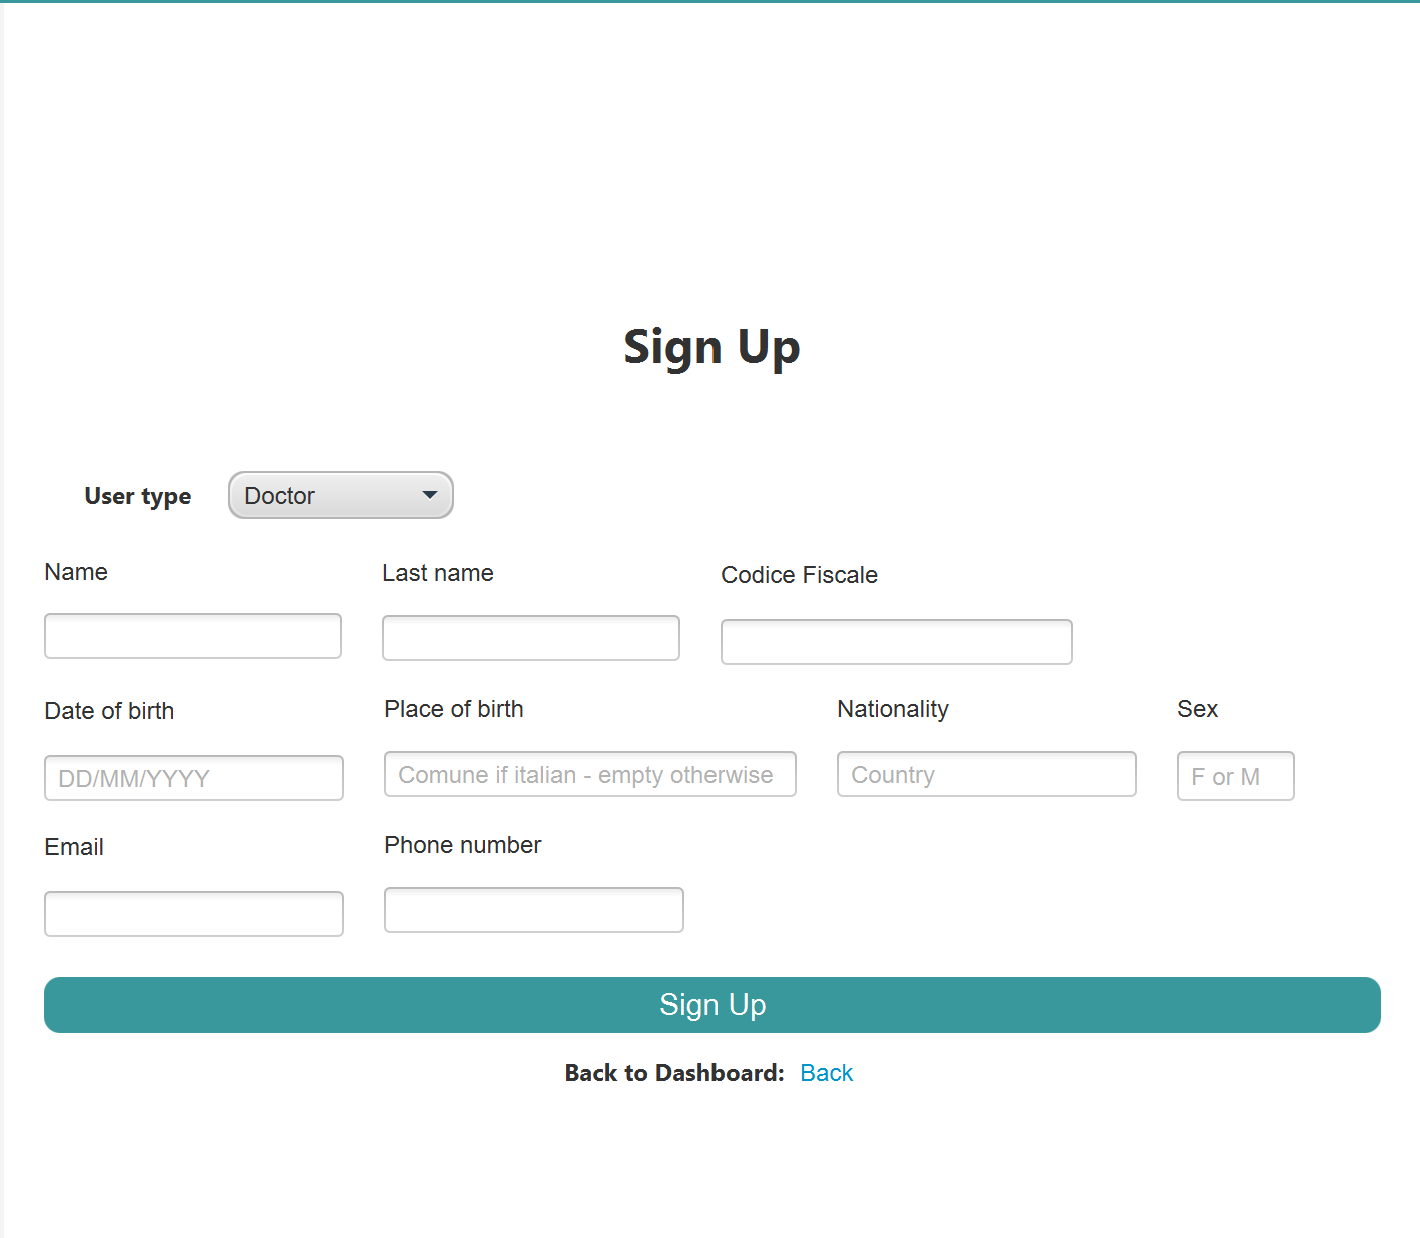
\includegraphics[width=0.9\linewidth, height=6cm]{doctor_signup_page.png} 
    \caption{Doctor sign up form}
    \label{fig:subim1}
    \end{subfigure}
    \begin{subfigure}{0.5\textwidth}
    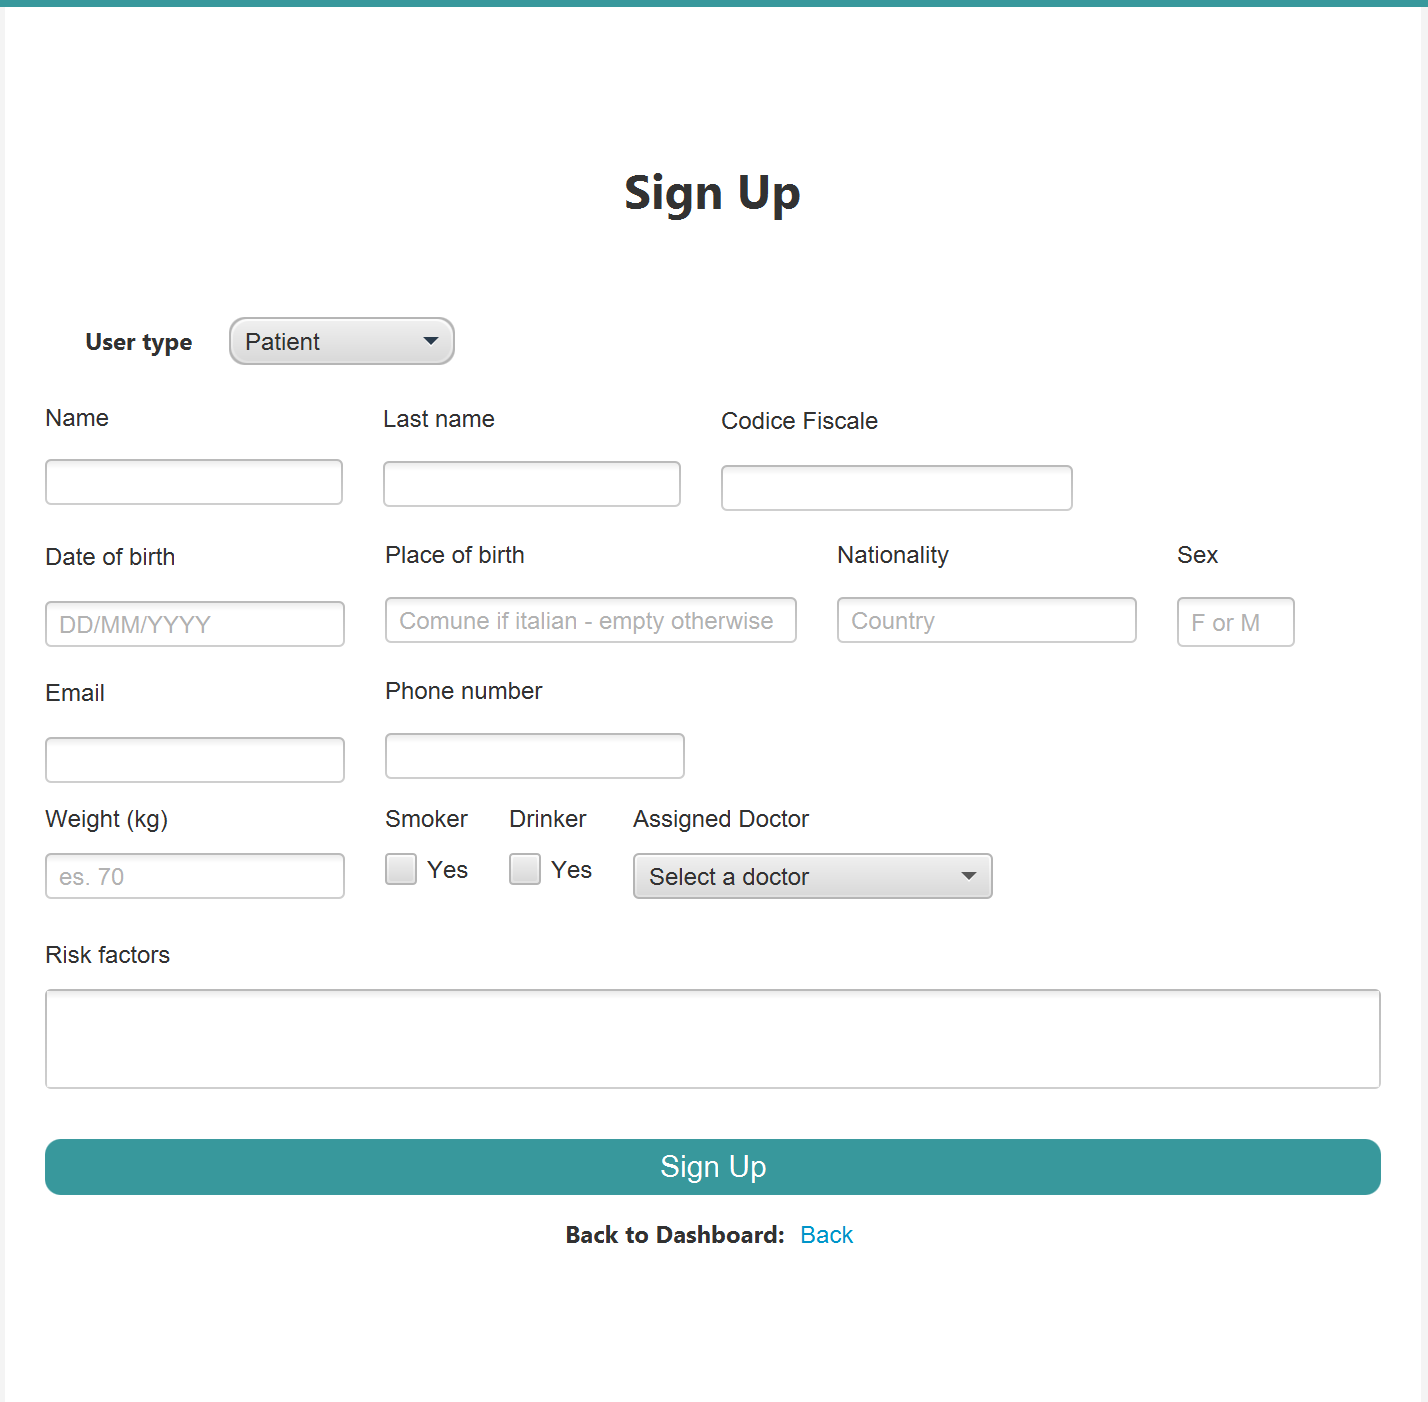
\includegraphics[width=0.9\linewidth, height=6cm]{patient_signup_page.png}
    \caption{Patient sing up form}
    \label{fig:subim2}
    \end{subfigure}
    \caption{User registration sections}
    \label{fig:image2}
    \end{figure}

    When signing up a user, in the 'place of birth' section you must write the comune of birth (in italian) if that person was born in Italy. If not leave it blank. In the 'nationality' field you must write the country (in italian). This is because the check function for the codice fiscale has a specific algorithm which uses dataset(for place of birth and nationality) retrieved from the official italian government website to calculate the codice fiscale. This algorithm is built using the official rules set by the italian government, though it may not be accurate since it is made from scratch.

    Insert all the needed information and click sign up. If everything is correct you'll see a success message and the user will receive an email with username and password. If you click delete, you will remove that user from the system. click back to dashboard to get back.

    If you click 'Doctor's activity log' you can see all variations made by all the doctors. Click view to see the detailed version.
    \begin{figure}[H]
        \centering
        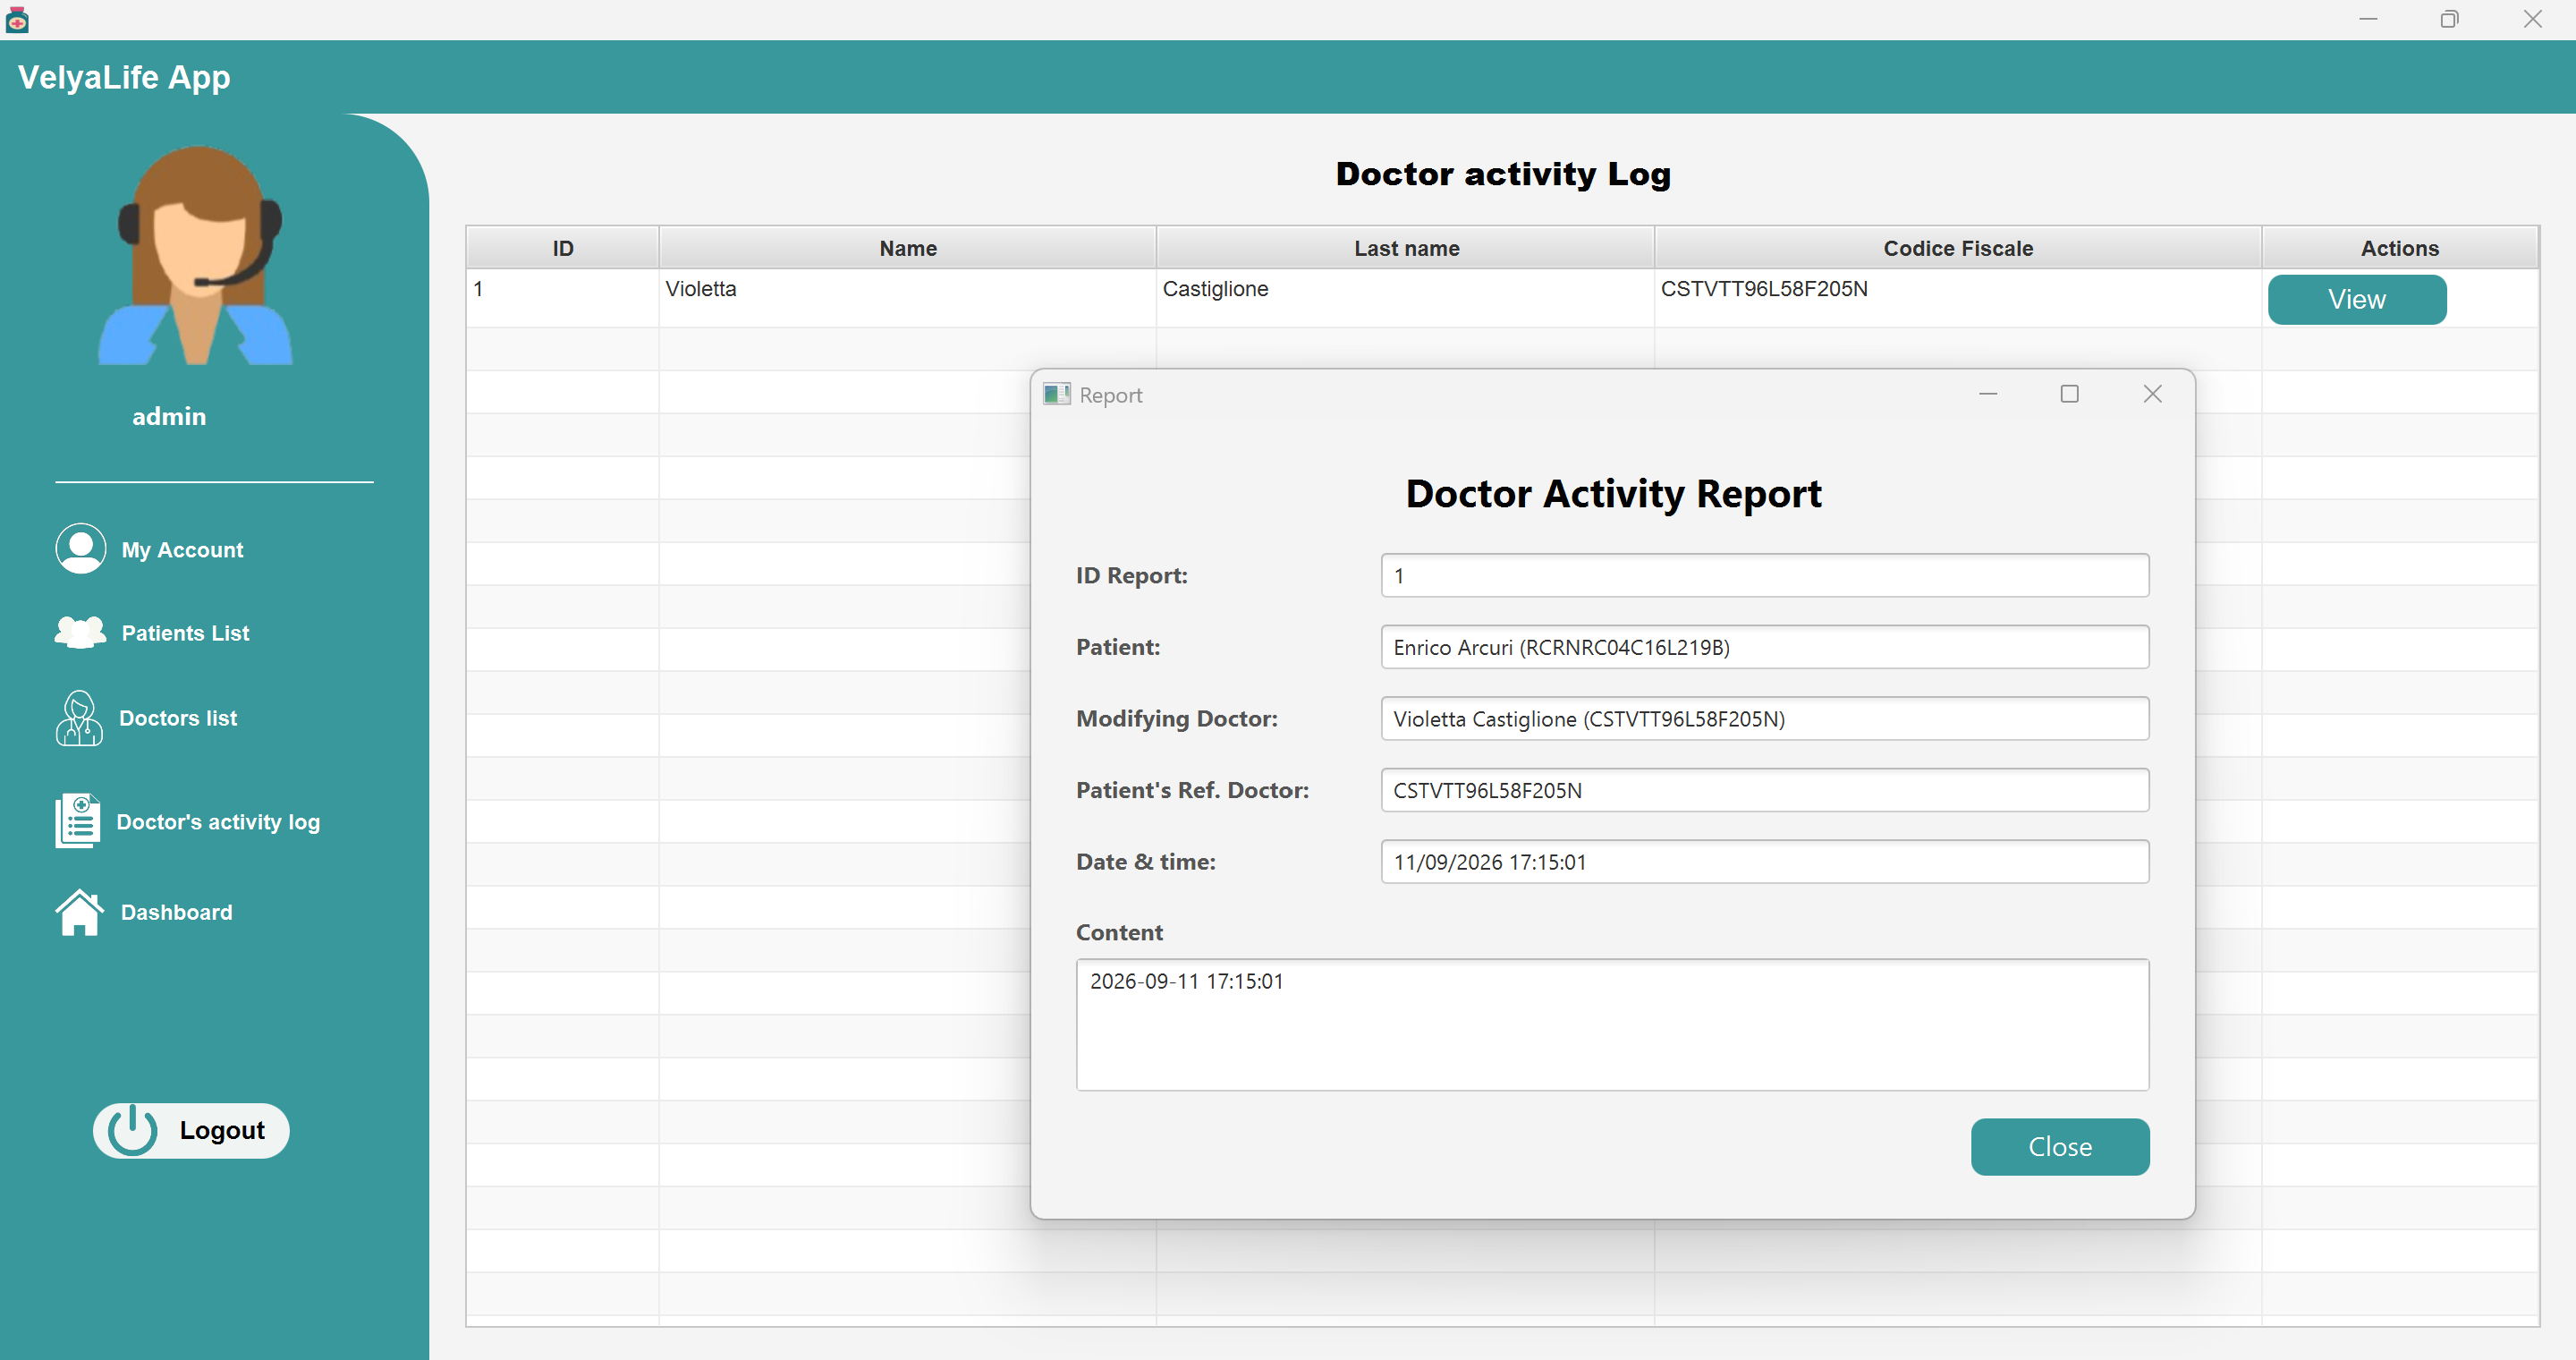
\includegraphics[width=1\linewidth]{doctor_activity_log_page.png}
        \caption{Doctor's activity}
    \end{figure}

    \subsubsection{Patient's dashboard}
    Patients can view all the messages they received in the 'messages' panel. Click view to see the details. In the contact page they'll find their primary doctor's information and the diabetes center's information.

    In the Daily Log page you can add your glycemic measurements, symptoms, other medical conditions and/or therapies. By clicking view you can see all the relative detail. You can also delete any log, though their are not retrievable.
    \begin{figure}[H]
        \centering
        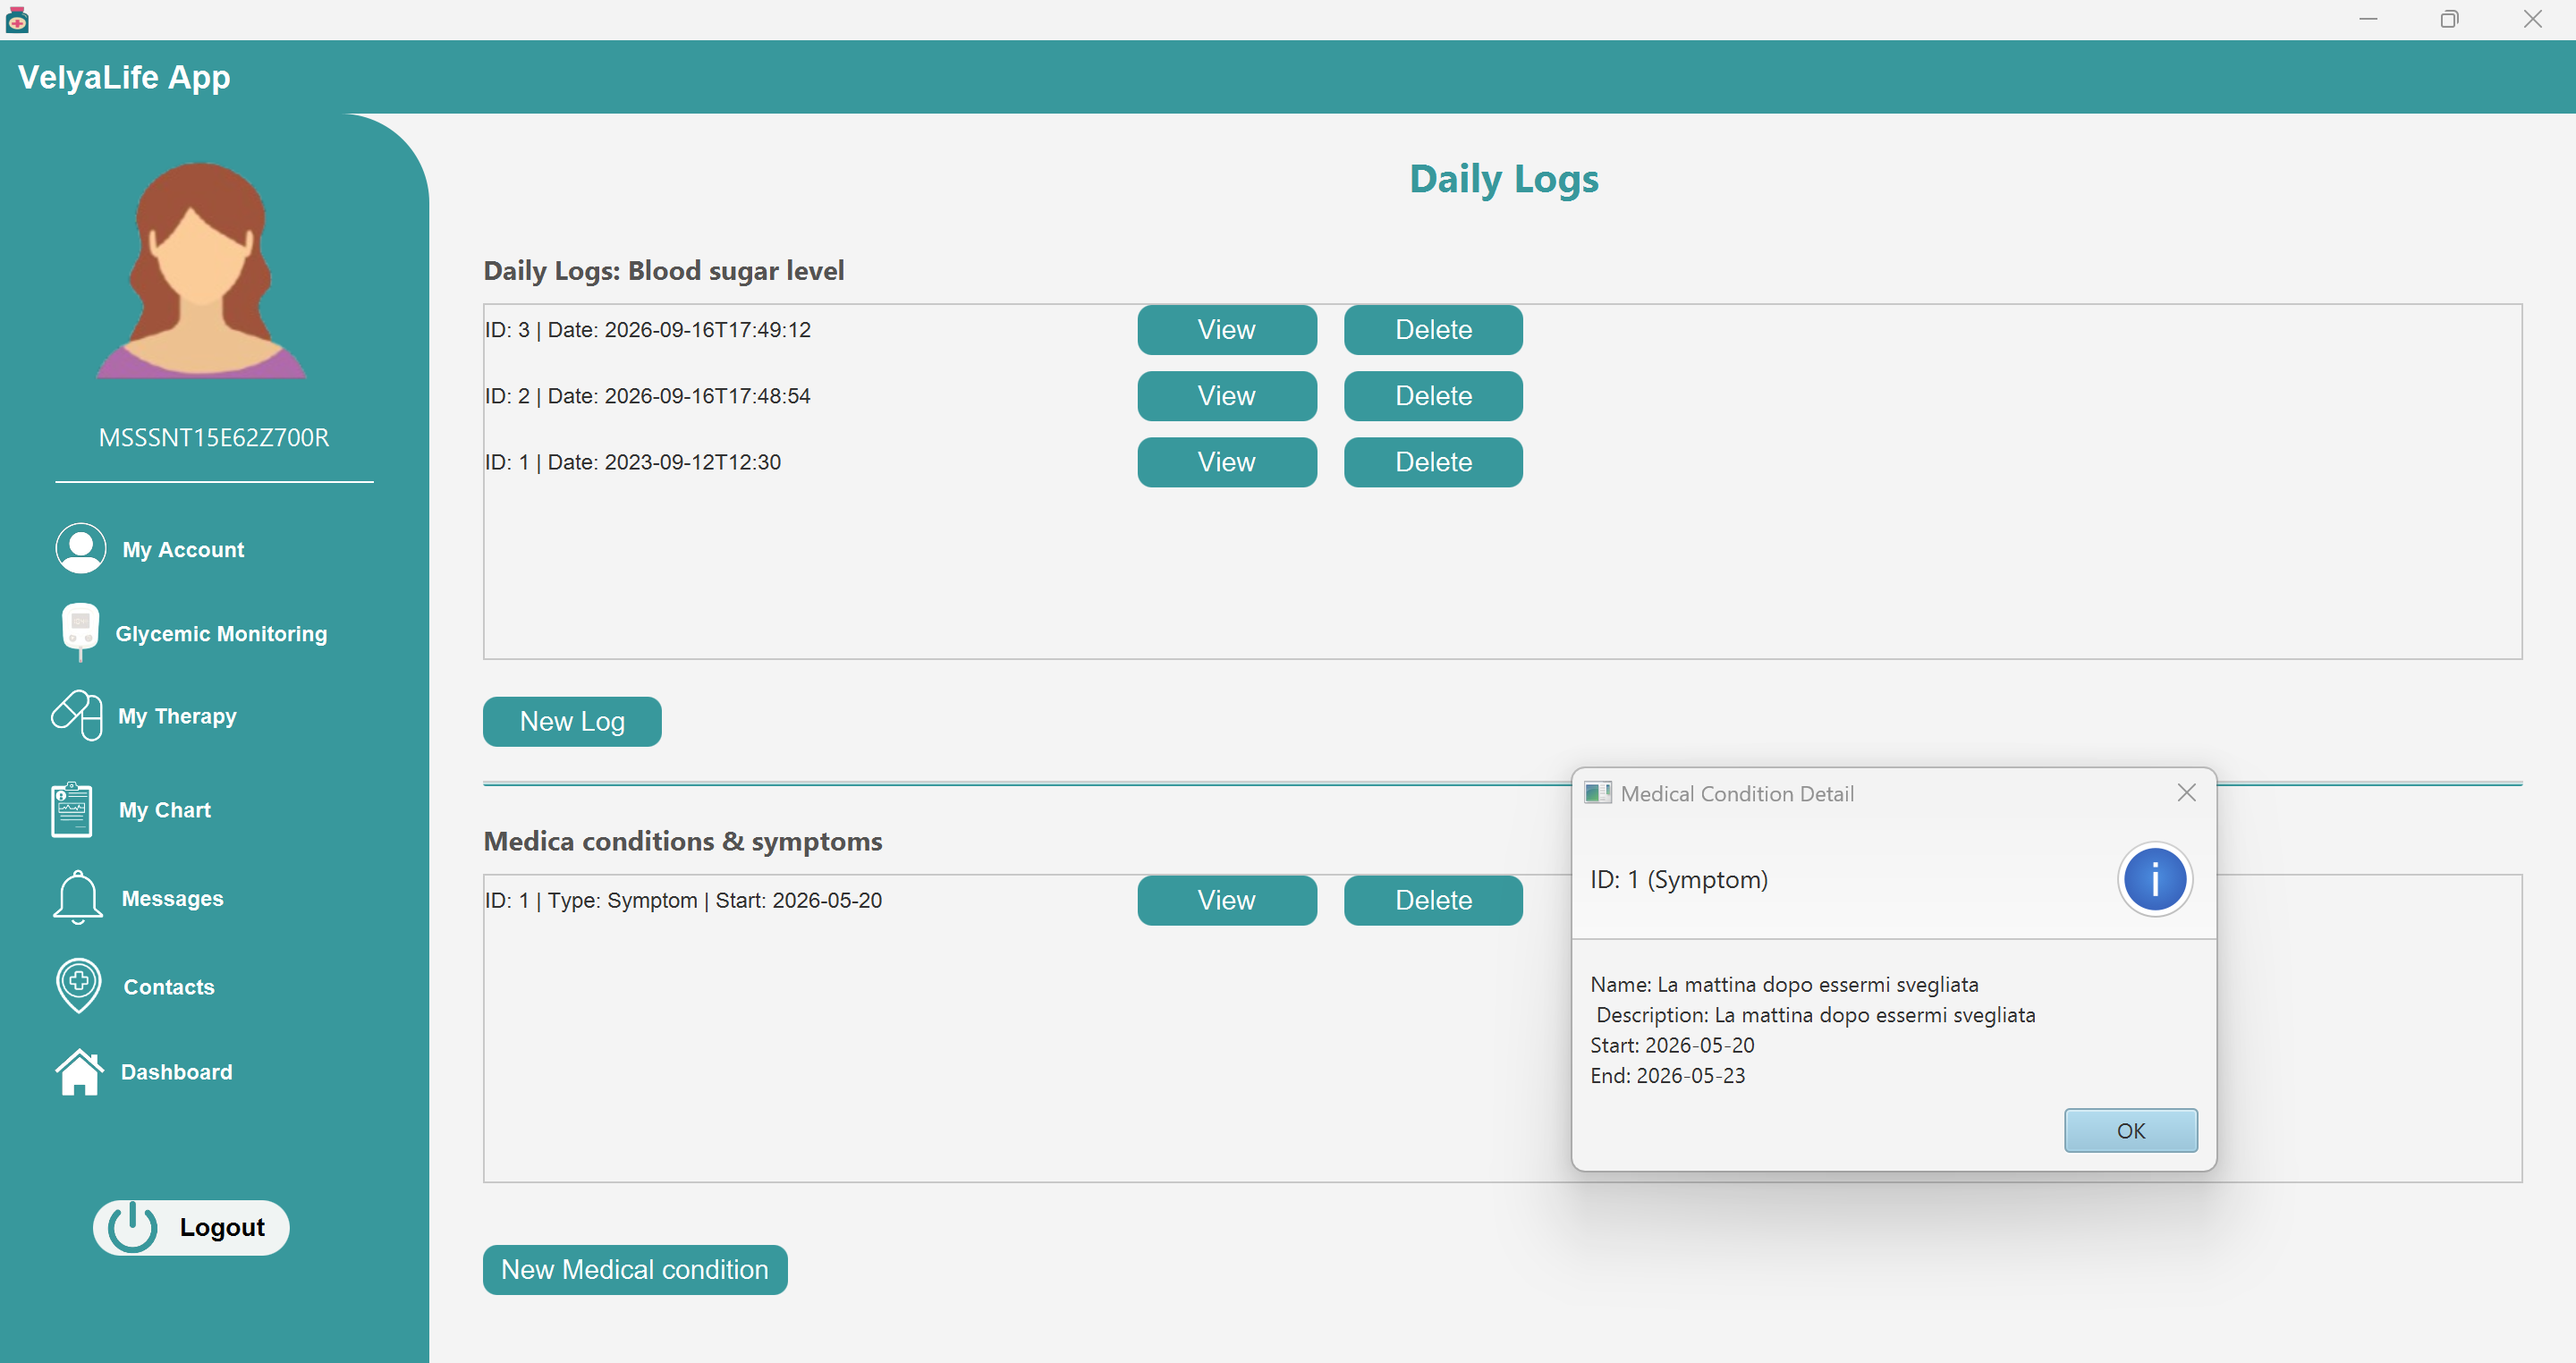
\includegraphics[width=1\linewidth]{dailyLog_page.png}
        \caption{Measurement page}
    \end{figure}

    By clicking 'My chart' you get a summary of your blood sugar lever. You can choose between the current day, week, month and year. On the right there is the list of all the glycemic measurements. Click download pdf to get the pdf version of this page on your desktop.
    \begin{figure}[H]
        \centering
        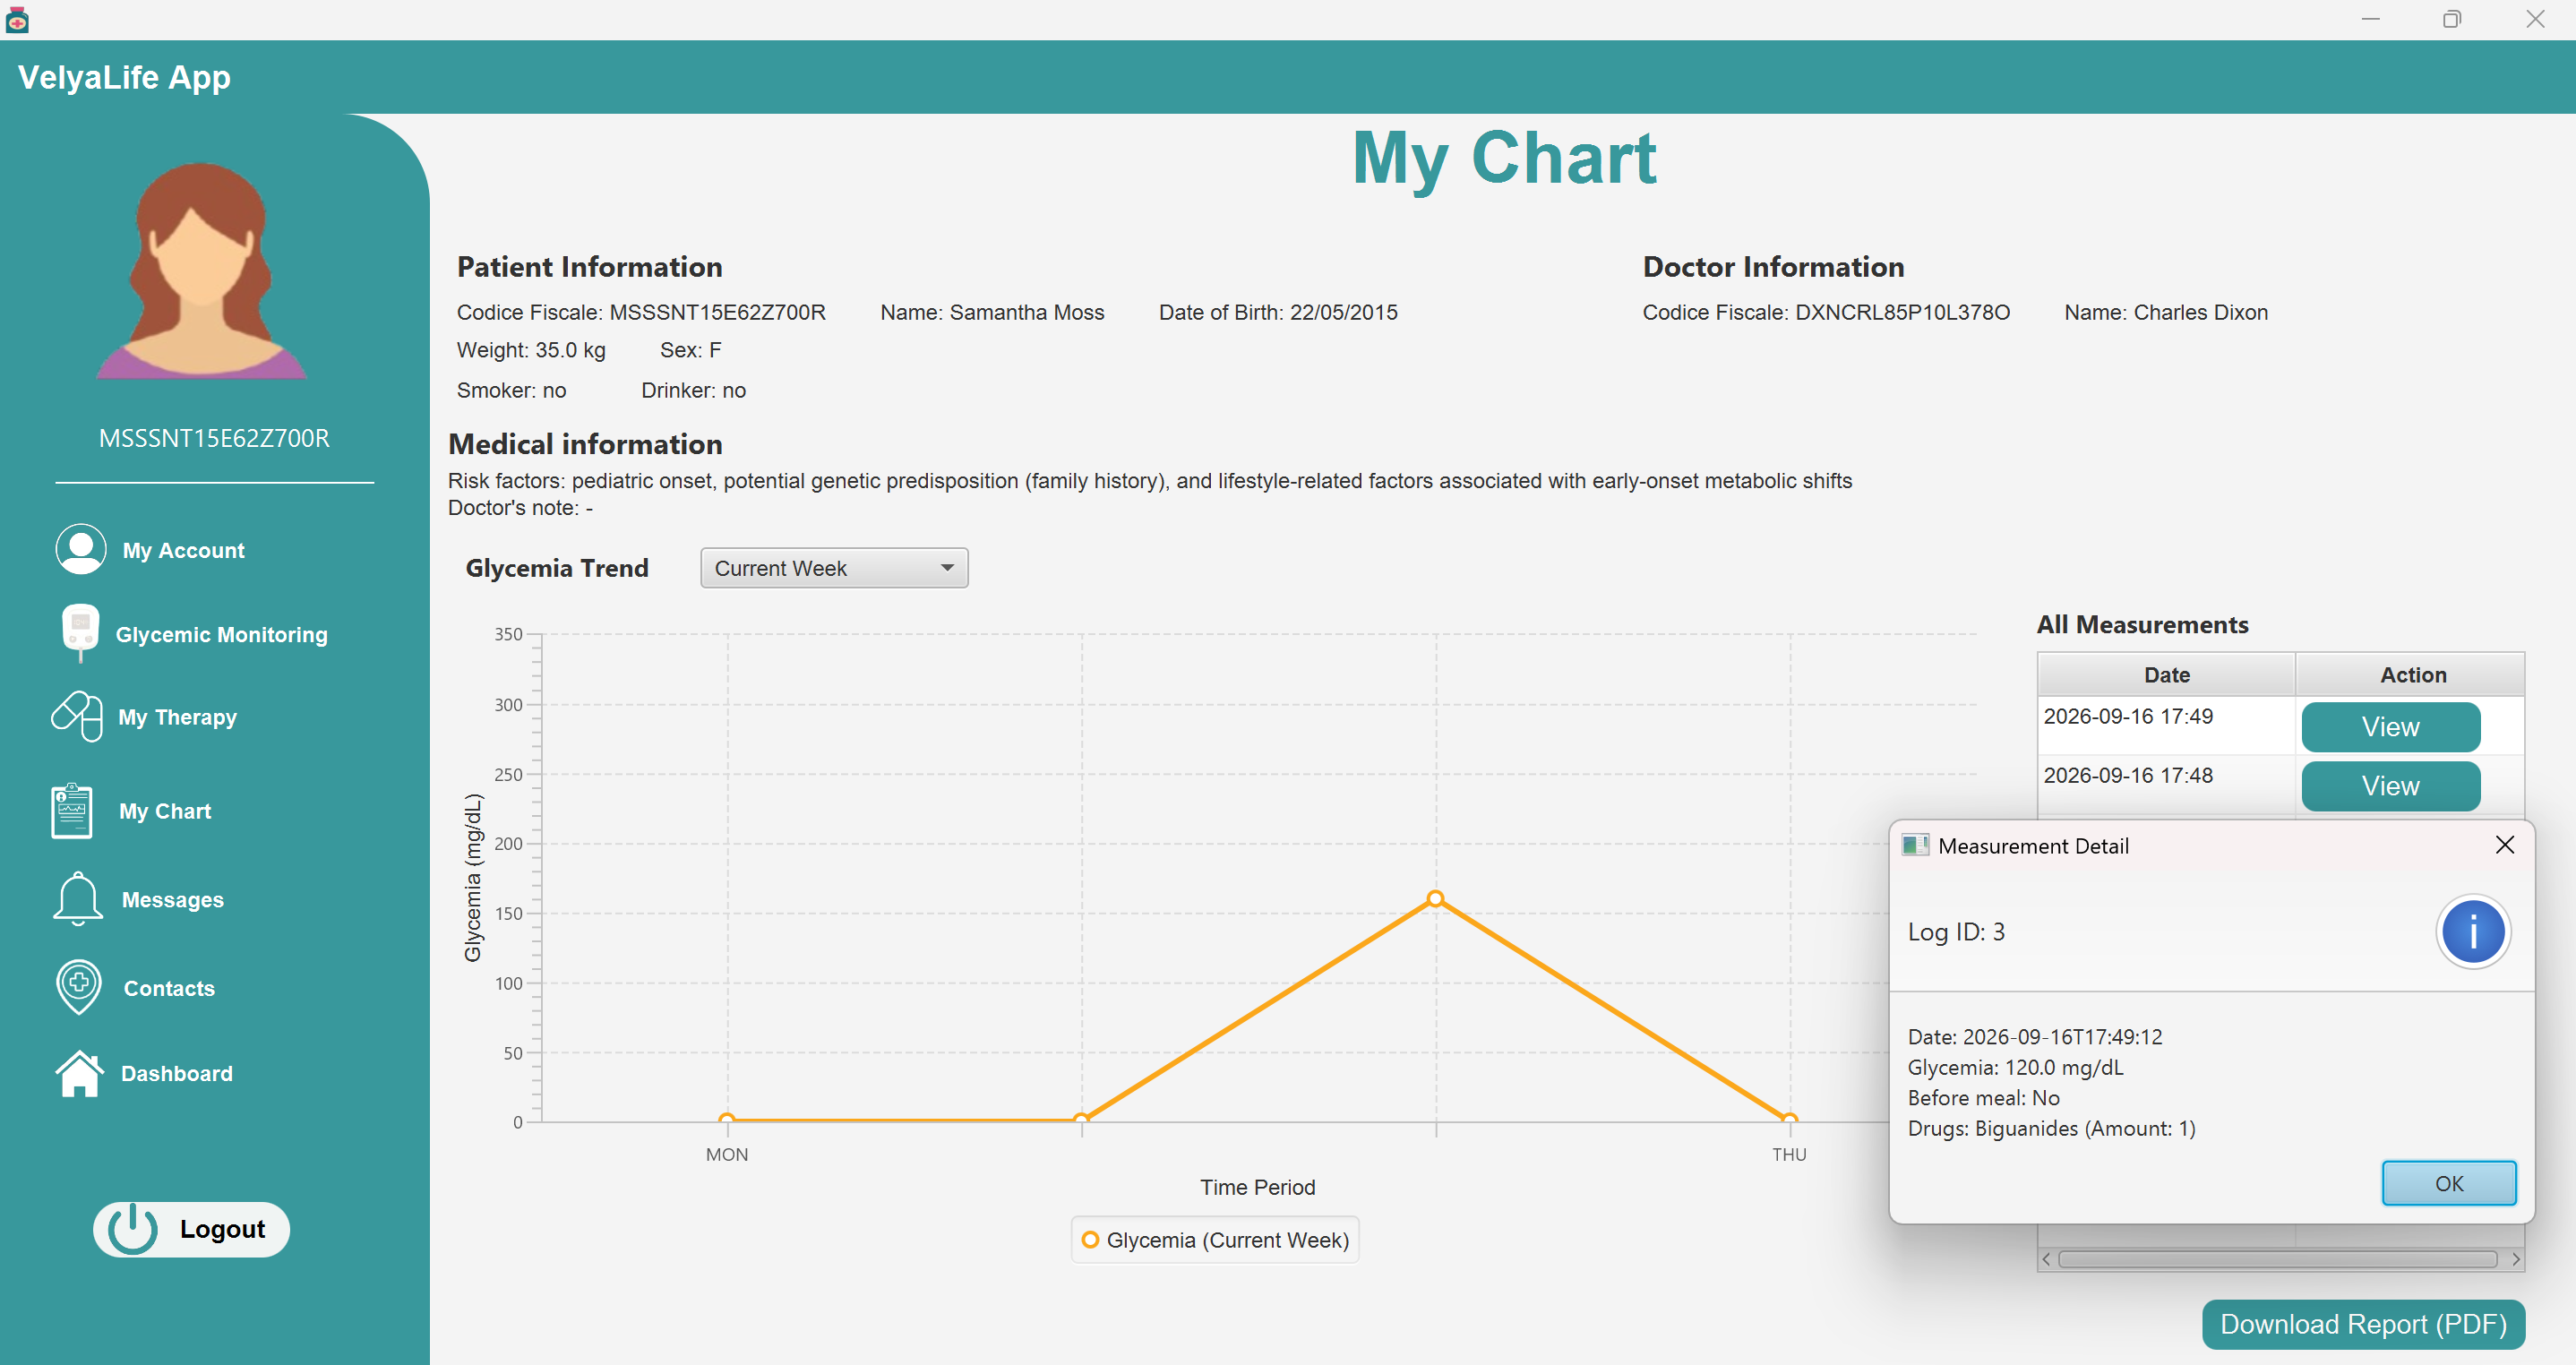
\includegraphics[width=1\linewidth]{patient_chart_page.png}
        \caption{Patient's chart page}
    \end{figure}

    In the therapy section there is the list of all the therapies assigned to that patient. The ones currently active have 'active' written in their status column. Click view to see the details.
    \begin{figure}[H]
        \centering
        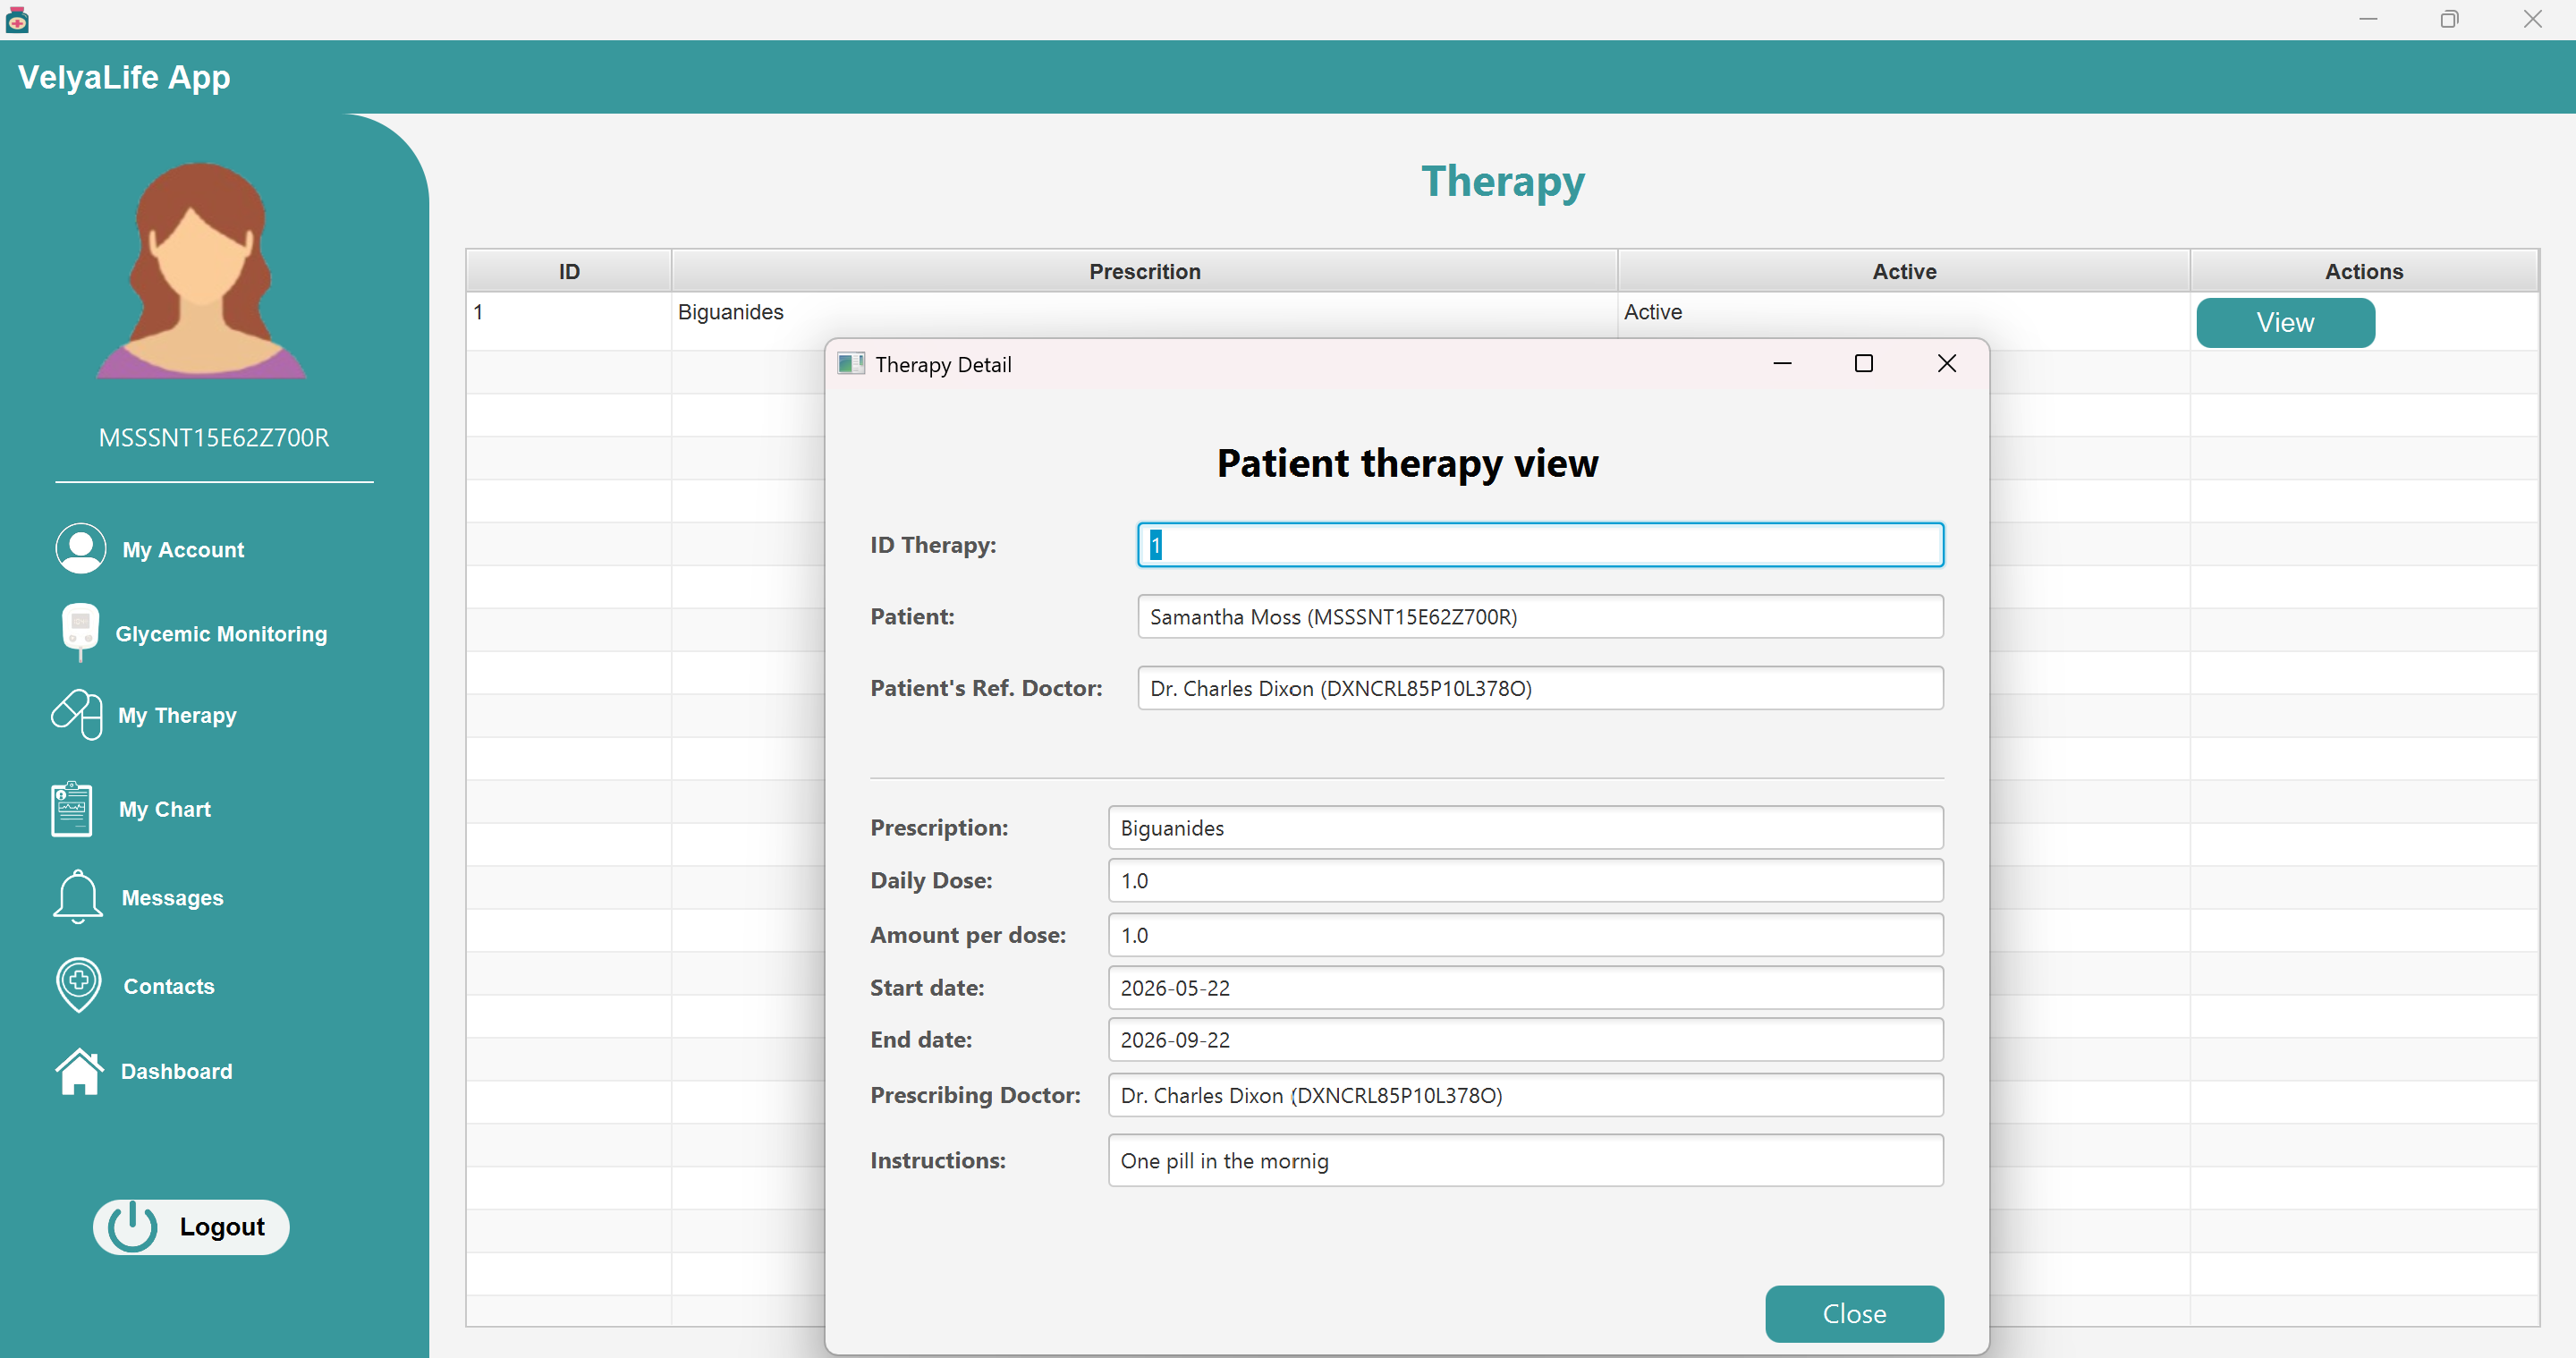
\includegraphics[width=1\linewidth]{therapy_page.png}
        \caption{Patient's chart page}
    \end{figure}

    \subsubsection{Doctor's dashboard}
    Notification, My account's pages are identical to the patient's shown before. In the patient's page there is a list of patients (one for the doctor's and one of all the patients of the center). By clicking view he can see the patients details, therapy, blood sugar levels measured.
    \begin{figure}[H]
        \centering
        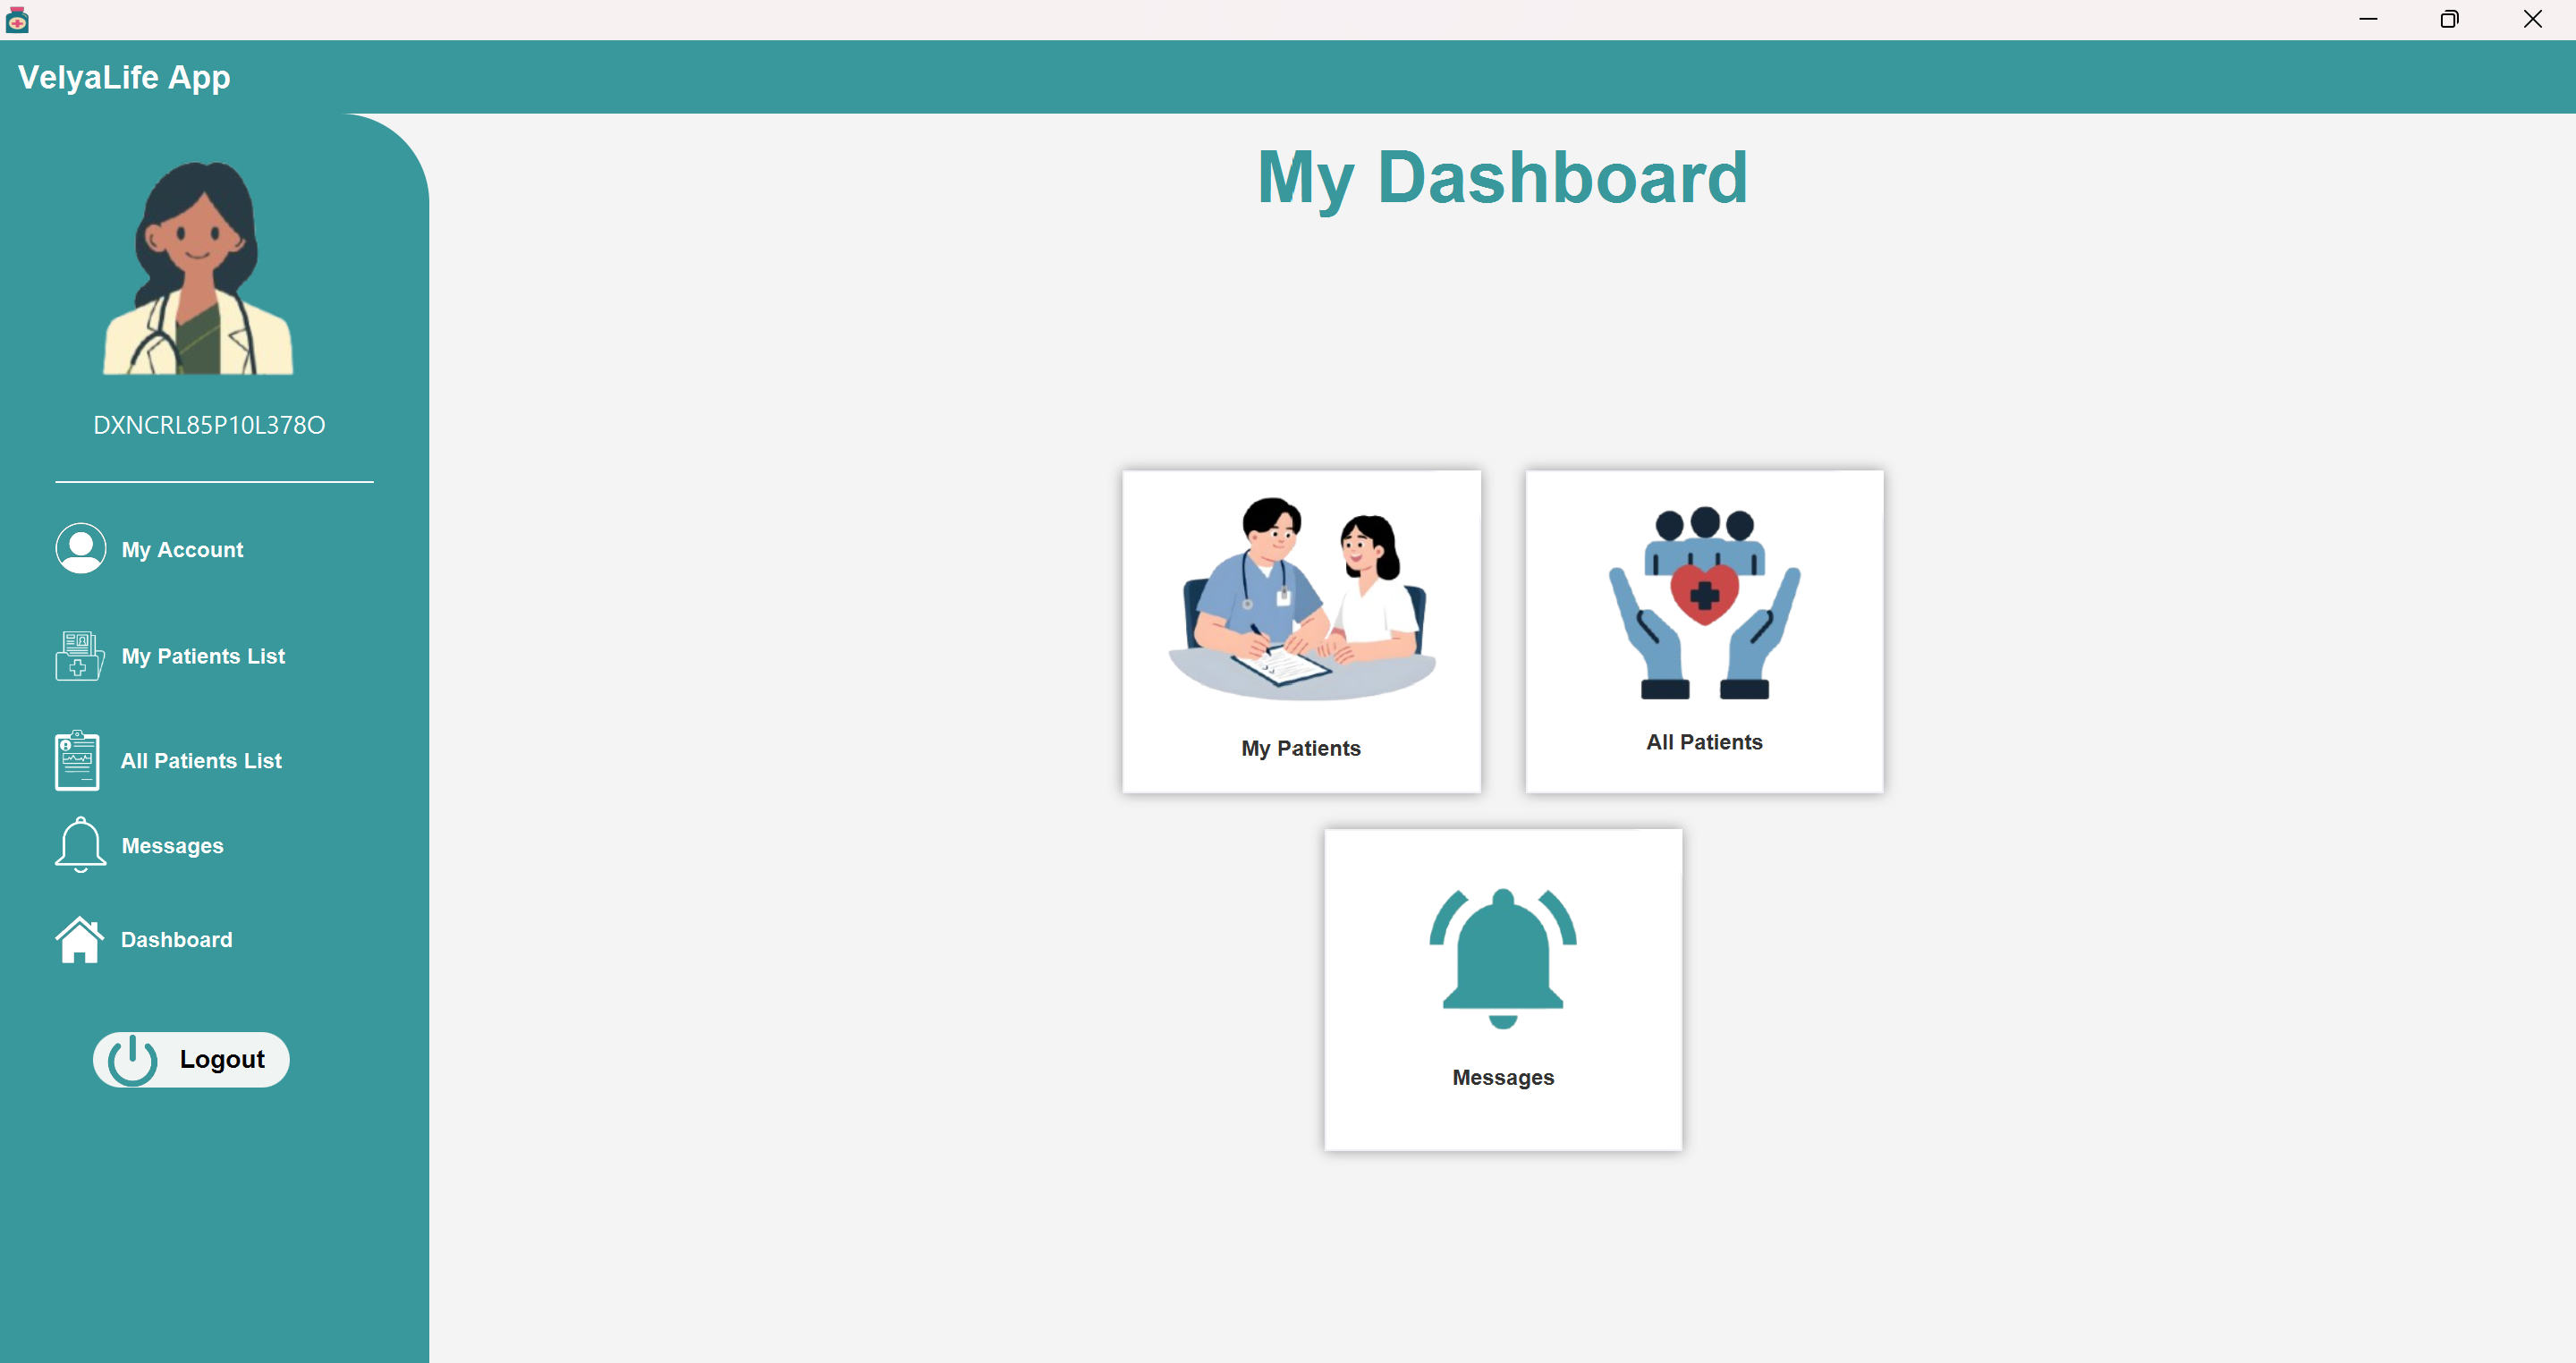
\includegraphics[width=1\linewidth]{doctor_dashboard_page.png}
        \caption{Doctor dashboard}
    \end{figure}

    \subsubsection{Patient's detail}
    All patients detail can be viewed in this page. There is a graph for the patient's sugar level based on their logs. There are also tables for thier medications, other medical conditions, and all doctor's modifications. At the end there is a download button to save this page on your pc. Any doctor can edit risk factors and doctor's note section and modify therapy. Only the doctor assigned for that patient can add or remove therapy. For any of these actions the patient receives a message.
    \begin{figure}[H]
        \centering
        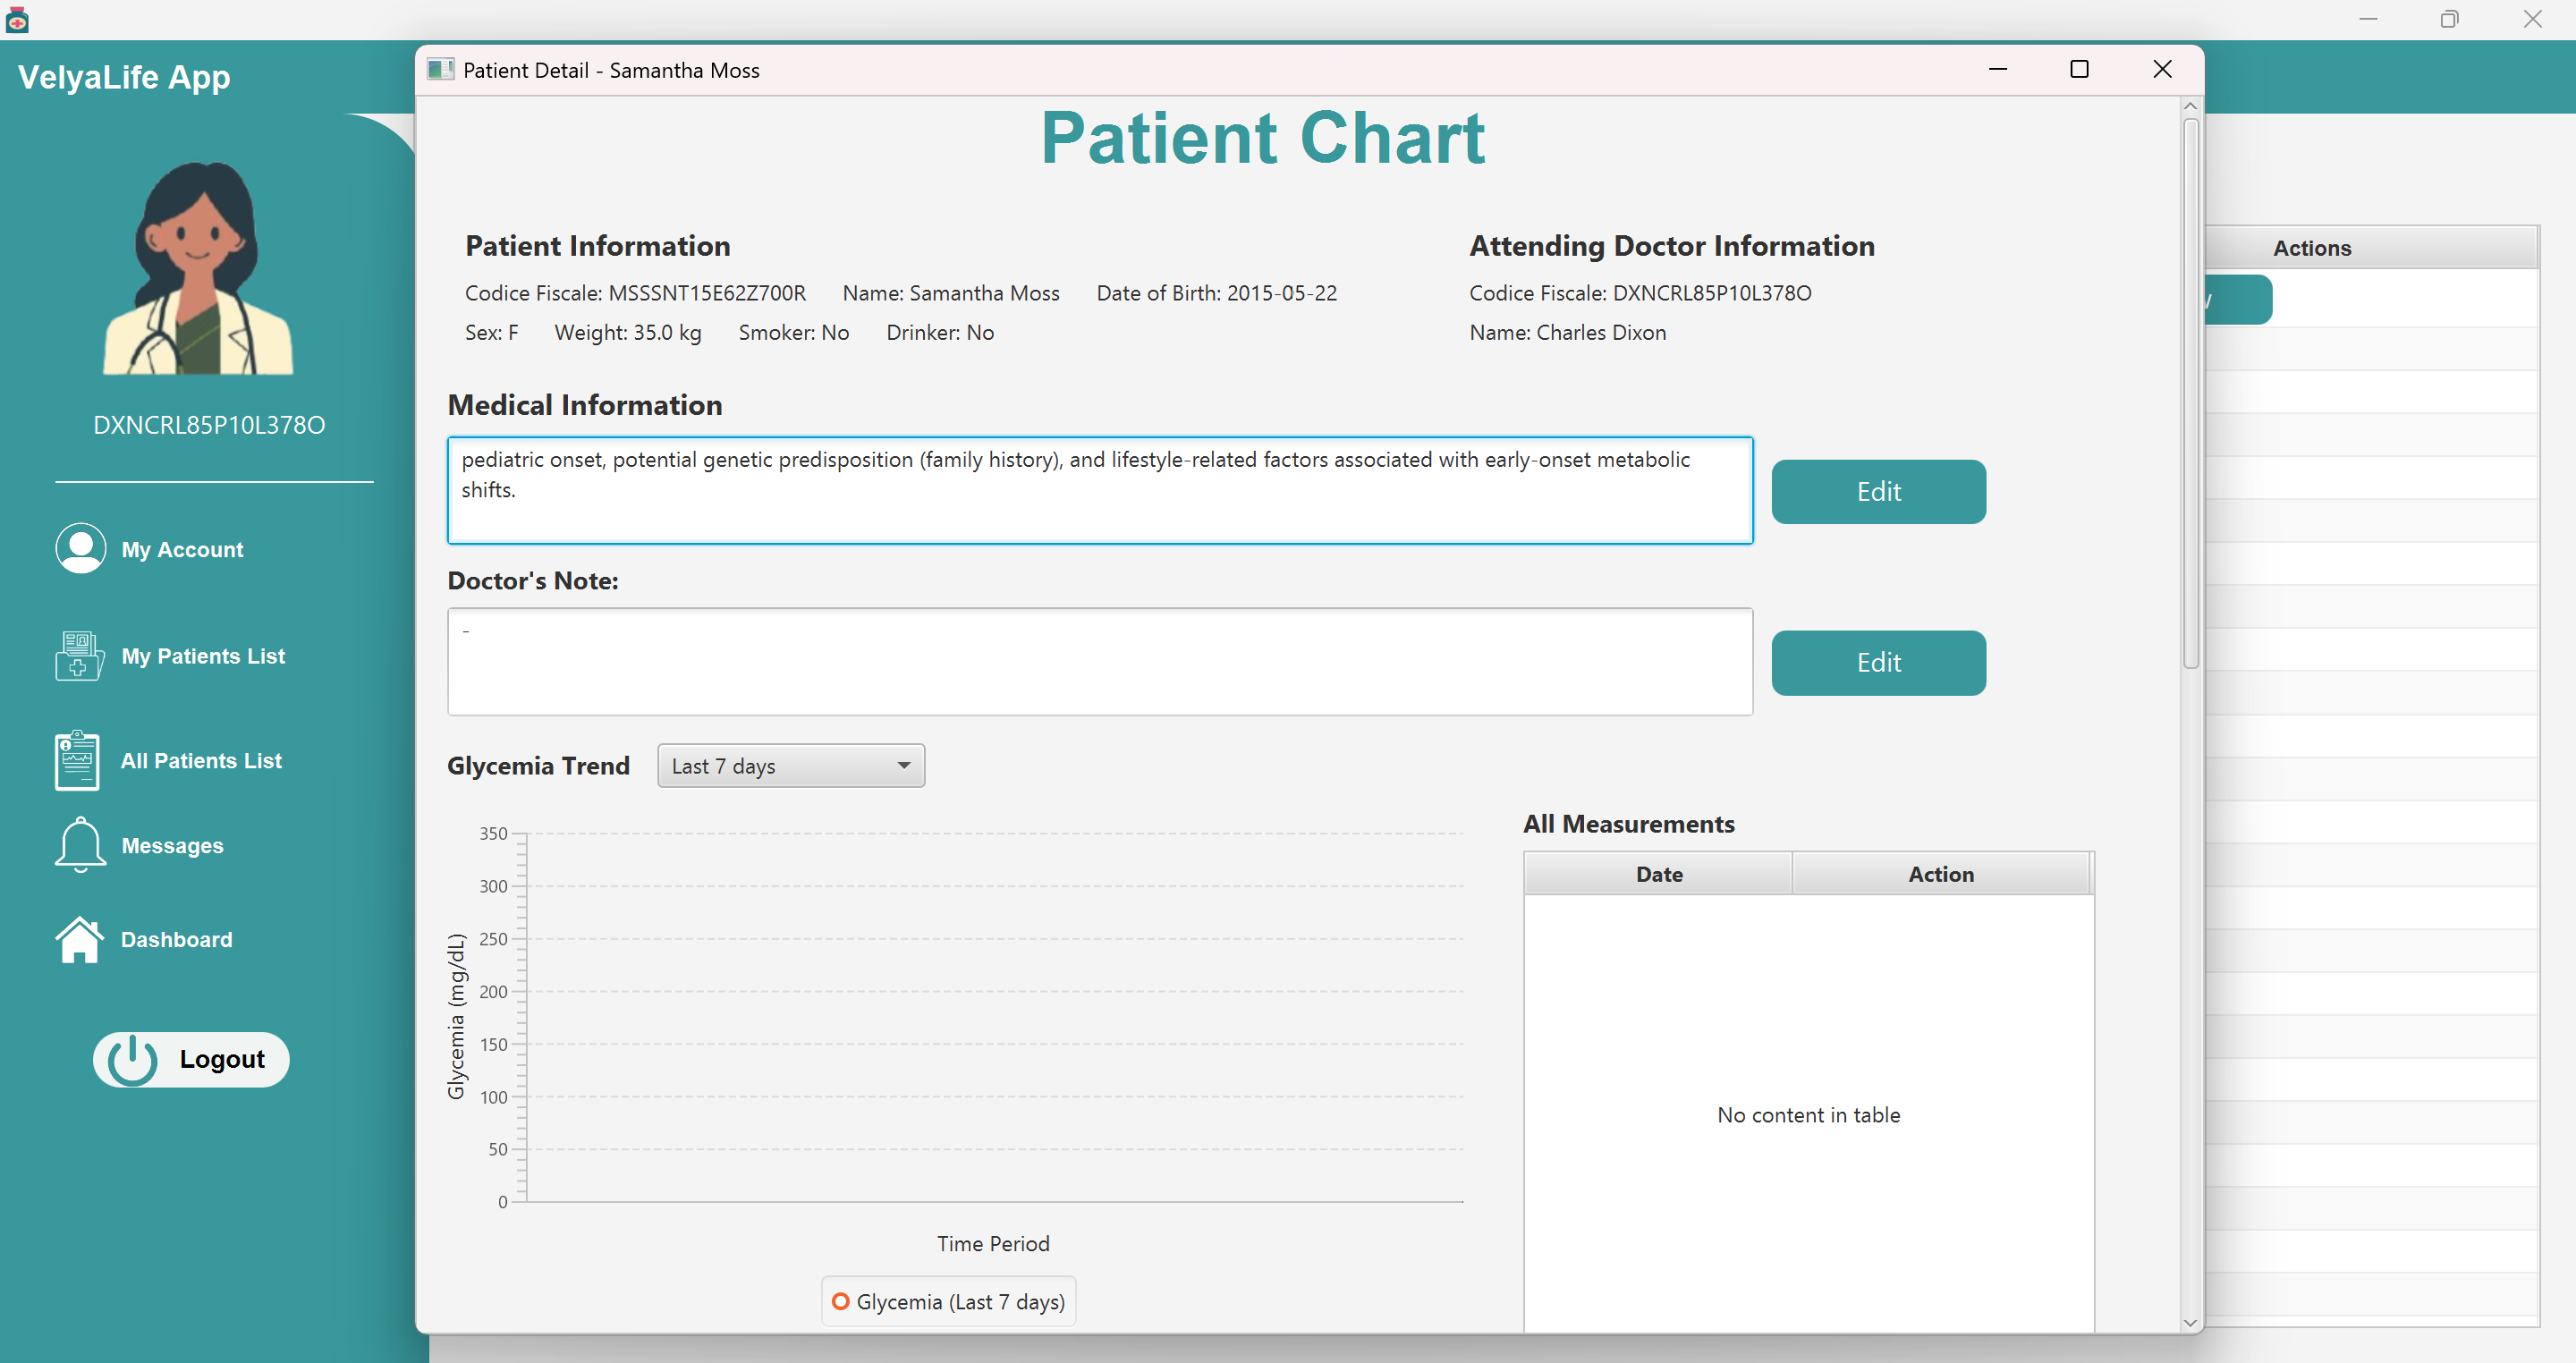
\includegraphics[width=1\linewidth]{patient_detail_page.png}
        \caption{Patient detail}
    \end{figure}

    \subsubsection{Alert system}
    When a patient logs their daily report, they will receive a remainder to correctly follow their therapy.
    \begin{figure}[H]
        \centering
        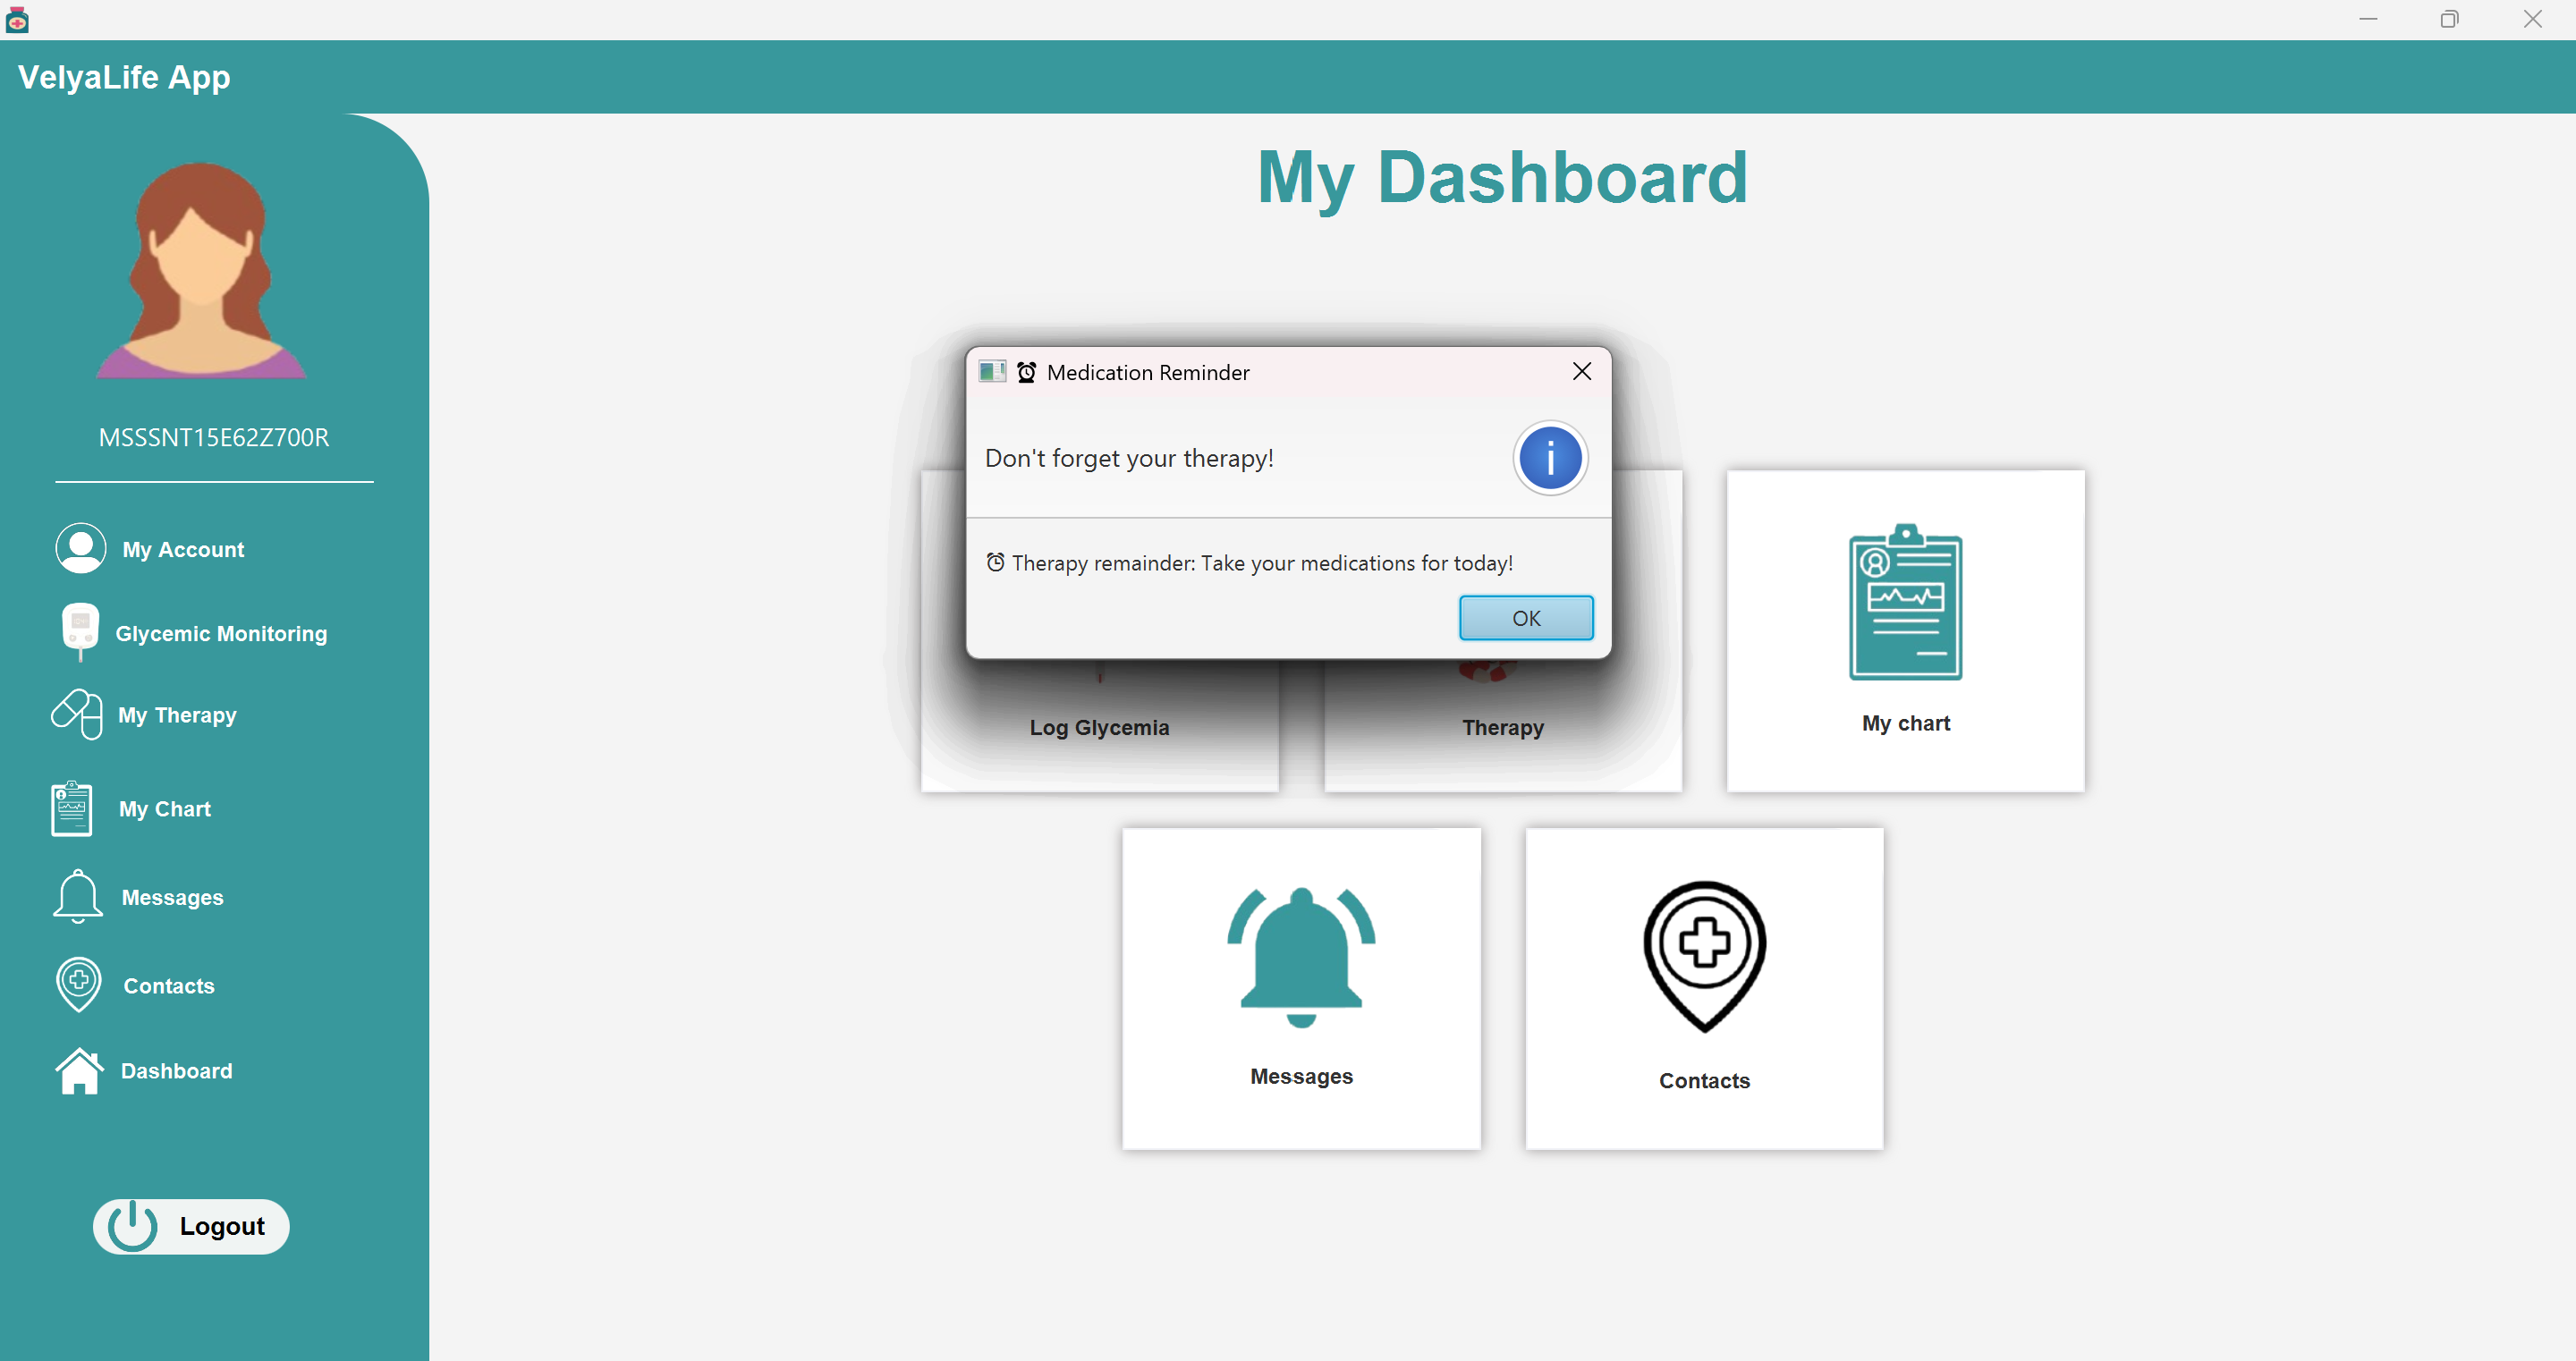
\includegraphics[width=1\linewidth]{patient_therapy_remainder.png}
        \caption{Patient Therapy remainder}
    \end{figure}

    If a patient registers unusual levels of blood sugar all doctors will be notified. They can decide to take care of that situation or let another doctor deal with it.
    \begin{figure}[H]
        \centering
        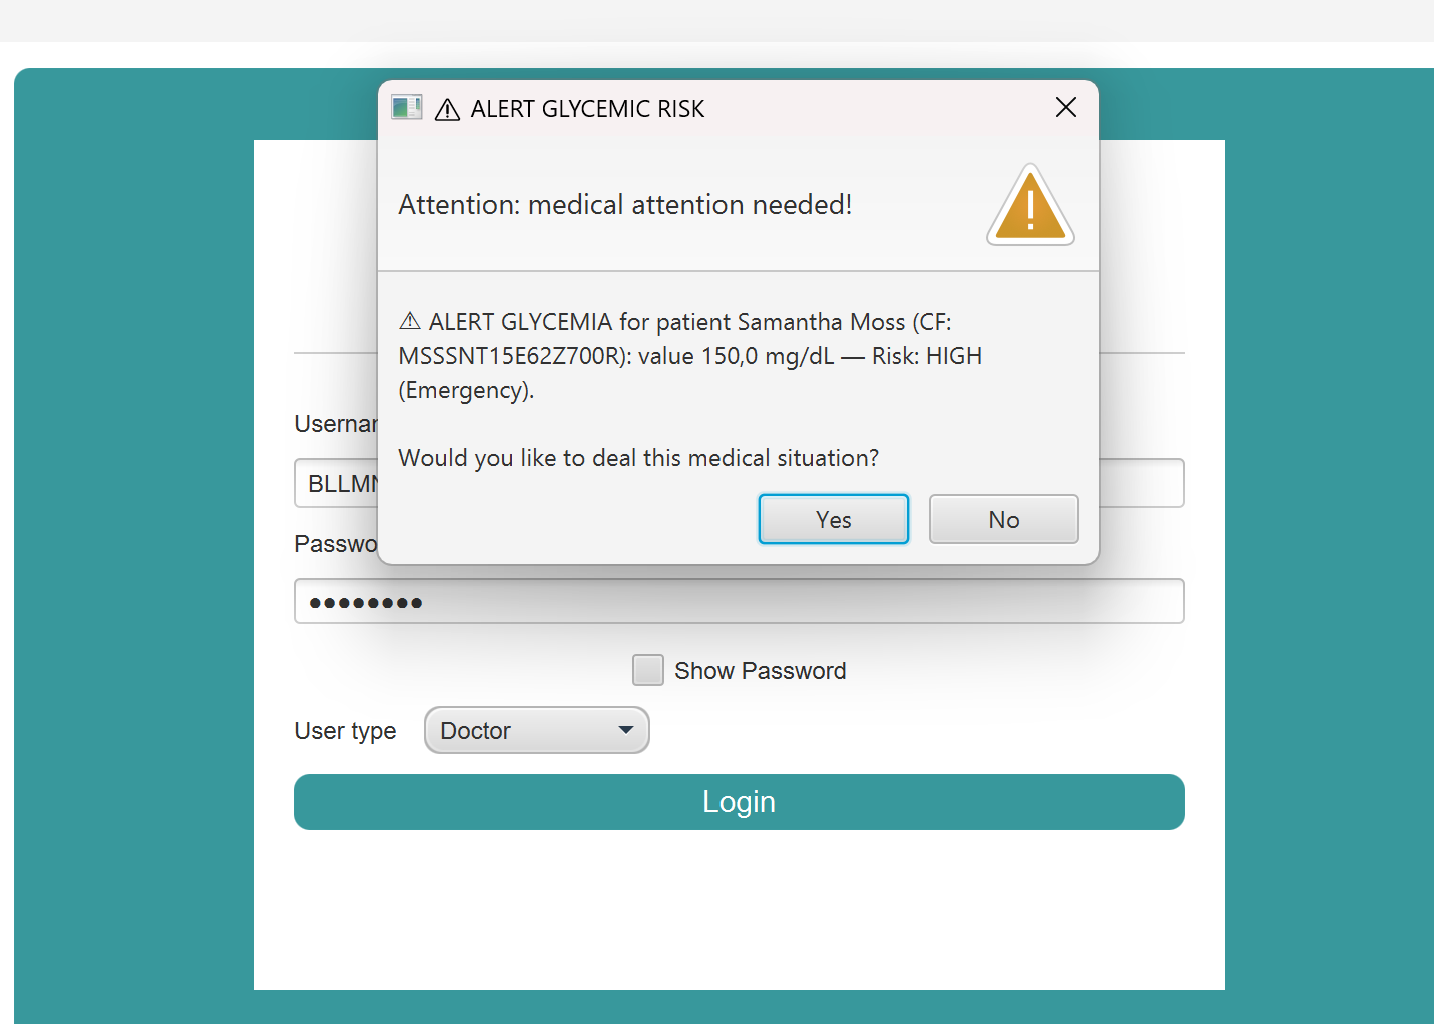
\includegraphics[width=1\linewidth]{glycemic_alert.png}
        \caption{Glycemia level alert}
    \end{figure}

    If a patient does not follow their therapy for three consecutive days, their assigned doctor receives an alert.
    \begin{figure}[H]
        \centering
        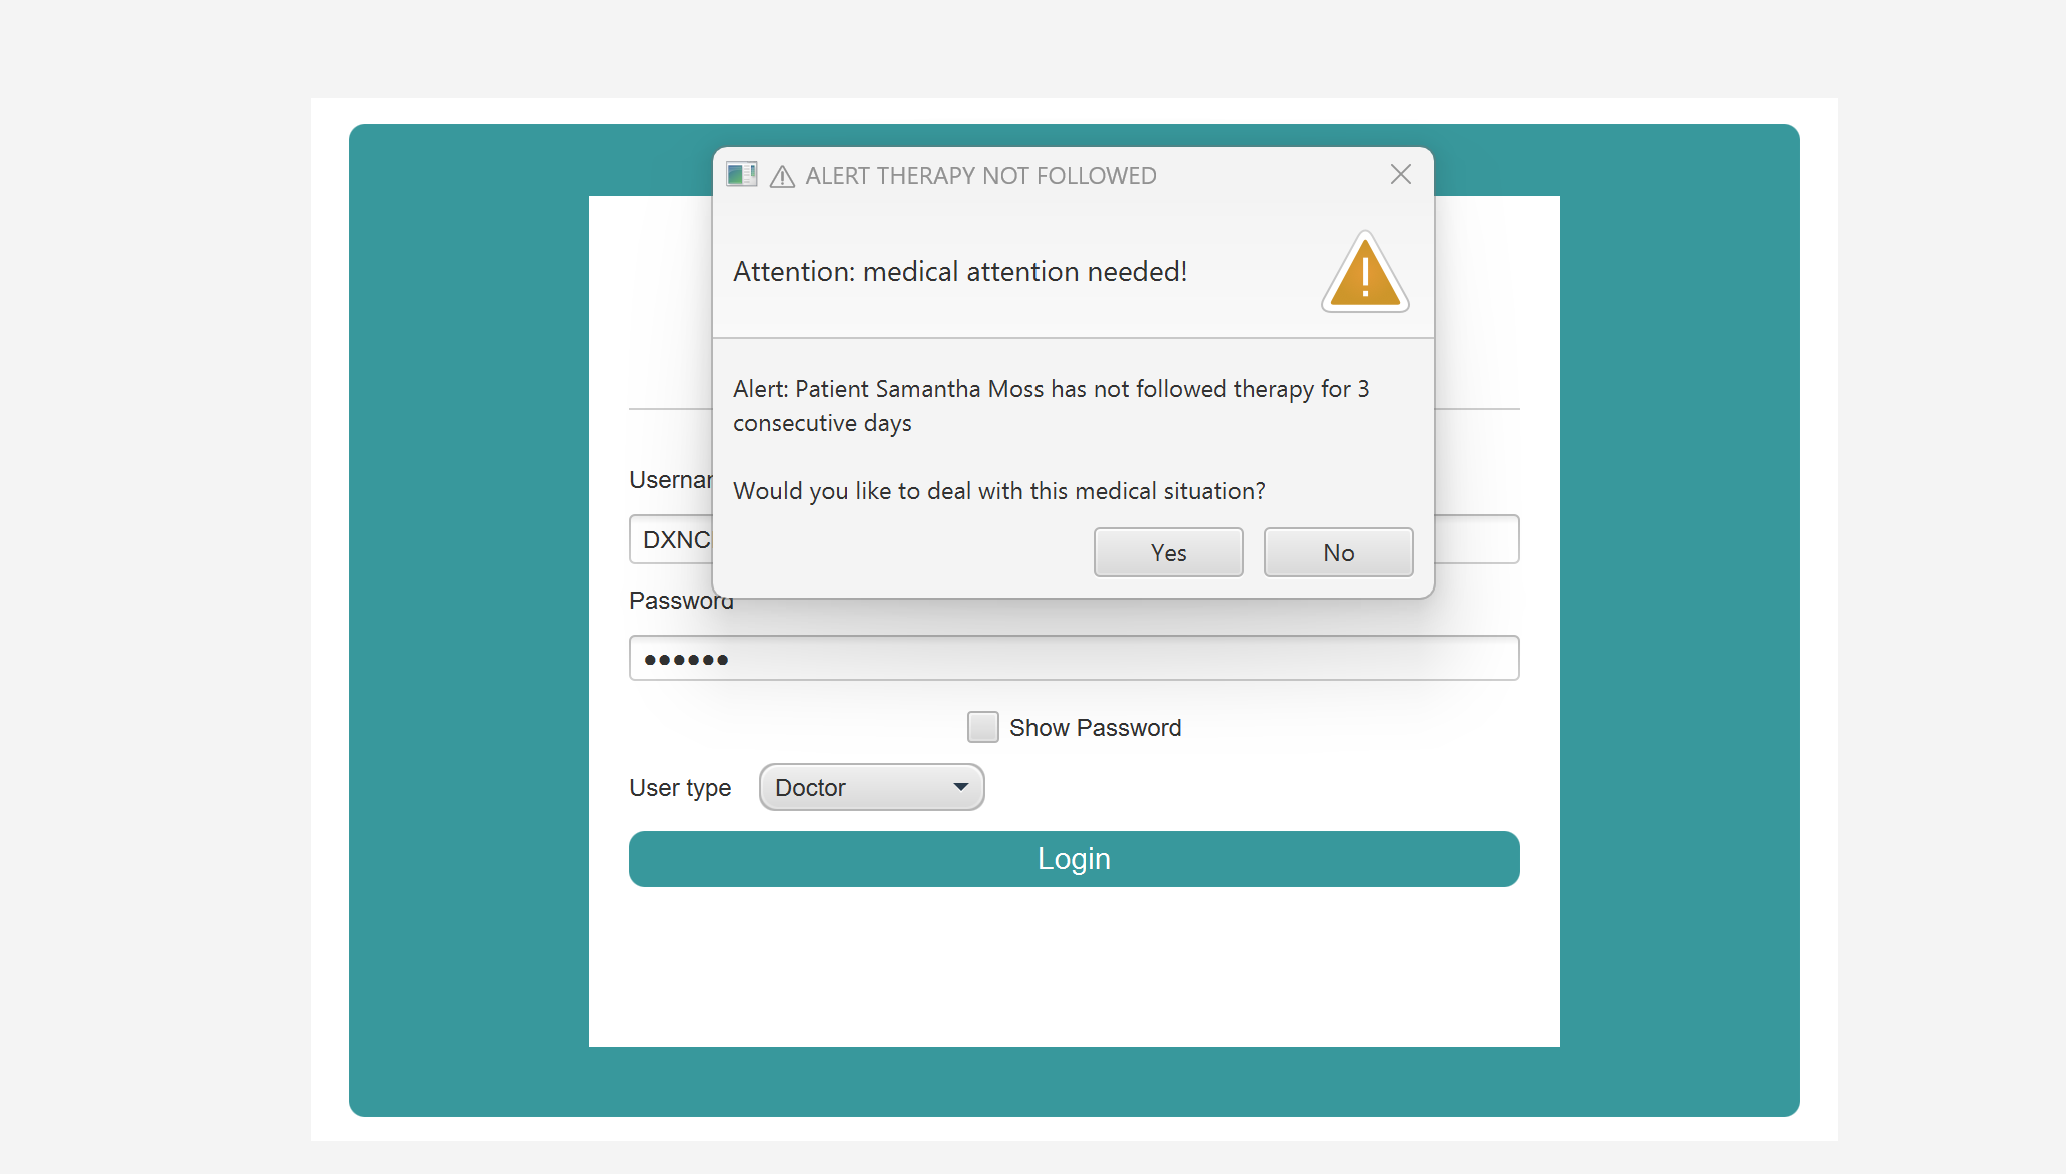
\includegraphics[width=1\linewidth]{therapy_not_followed.png}
        \caption{Therapy not followed for three days}
    \end{figure}                                                                                                                               
    \newpage
    \section{Resources}
    \label{resources}
    \begin{itemize}
        \item Intellij setup documentation:
        \begin{itemize}
            \item \url{https://www.jetbrains.com/help/idea/installation-guide.html#requirements}
        \end{itemize}
        \item Configure intellij for java:
        \begin{itemize}
            \item \url{https://www.jetbrains.com/help/idea/creating-and-running-your-first-java-application.html#create-project}
        \end{itemize}
        \item JavaFx setup:
        \begin{itemize}
            \item \url{https://www.jetbrains.com/help/idea/javafx.html#create-project}
        \end{itemize}
        \item SQLite:
        \begin{itemize}
            \item \url{https://sqlite.org/}
            \item \url{https://www.jetbrains.com/help/idea/quick-start-with-database-functionality.html}
        \end{itemize}
        \item DB Browser for SQLite:
        \begin{itemize}
            \item \url{https://sqlitebrowser.org/}
        \end{itemize}
        \item Canva: \url{https://www.canva.com/en_gb/}
        \item Generate codice fiscale: \url{https://www.codicefiscaleonline.com/?refresh_ce}
        \item Jakartamail for email:
        \begin{itemize}
            \item \url{https://mvnrepository.com/artifact/jakarta.mail/jakarta.mail-api}
        \end{itemize}
    \end{itemize}   
\end{document}